\documentclass[11pt,twoside,openany]{report}
\newcommand{\TemplateVersion}{1.0.0}
\newcommand{\PDFBookTitle}{Математический анализ. Часть I}
\newcommand{\PDFBookAuthor}{X.~Y.~Zettov, И.~И.~Иванов}
\newcommand{\PDFBookSubject}{Учебник по математическому анализу}
\newcommand{\PDFBookKeywords}{математический анализ, учебник}
\usepackage{xcolor}


% =============================================================================
% Базовые цвета
% =============================================================================

\definecolor{xblue}{HTML}{3182CE}
\definecolor{xgray}{HTML}{718096}
\definecolor{xgreen}{HTML}{38A169}
\definecolor{xindigo}{HTML}{3C40A0}
\definecolor{xmoss}{HTML}{5D715E}
\definecolor{xolive}{HTML}{5F7A1E}
\definecolor{xorange}{HTML}{DD6B20}
\definecolor{xpink}{HTML}{D53F8C}
\definecolor{xpurple}{HTML}{6B46C1}
\definecolor{xred}{HTML}{B03030}
\definecolor{xrust}{HTML}{9C4221} 
\definecolor{xsepia}{HTML}{8B5E3C}
\definecolor{xstone}{HTML}{999999}


% =============================================================================
% Цвета определений, утверждений, лемм, теорем, и т.п.
% =============================================================================

\colorlet{deficolor}{xblue}
\colorlet{statcolor}{xgreen!85!black}
\colorlet{lemmcolor}{xgray}
\colorlet{theocolor}{xpurple}
\colorlet{conccolor}{xolive!65!black}
\colorlet{examcolor}{xsepia!80!white}
\colorlet{notecolor}{xpink!80}
\colorlet{algocolor}{xrust!40!black}
\colorlet{codecolor}{xindigo!30!black}
\colorlet{taskanswercolor}{xblue!85!black}


% =============================================================================
% Цвета маркеров дополнительного материала
% =============================================================================

\colorlet{optionalmarkstarTop}{xorange!42!white}
\colorlet{optionalmarkstarBottom}{xorange!78!xrust}
\colorlet{optionalmarkstarFrame}{xrust!85!black}
\colorlet{optionalmarkaccent}{xrust!72!xorange}
\colorlet{optionalmarkline}{xorange!68!xrust}


% =============================================================================
% Цвета списков
% =============================================================================

\colorlet{listL1}{xred!70!black}
\colorlet{listL2}{xred!55!black}
\colorlet{listL3}{xred!40!black}


% =============================================================================
% Цвета todo-шек
% =============================================================================

\colorlet{todobackground}{xorange!20}     % Светло-оранжевый фон
\colorlet{todoborder}{xorange}            % Оранжевая рамка


% =============================================================================
% Специальные цвета
% =============================================================================

\colorlet{xcovere}{xmoss}                     % Цвет на обложке
\colorlet{xmatrix}{xmoss}                     % Базовый «матричный» зелёный
\colorlet{xmatrixDark}{xmoss!75!black}        % Тёмный оттенок для текста
\colorlet{xmatrixGlow}{xmoss!40}              % Полупрозрачный для «свечения»
\colorlet{blockreftext}{xindigo!62!black}     % Текст именованной ссылки
\colorlet{blockrefback}{xindigo!7!white}      % Фон номерного бейджа
\colorlet{blockrefframe}{xindigo!28!white}    % Рамка номерного бейджа
% =============================================================================
% ---> Геометрия страницы
% =============================================================================

\usepackage[
  papersize={170mm,240mm},
  inner=18mm,
  outer=20mm,
  bindingoffset=10mm,
  top=25mm,
  bottom=28mm,
  headheight=0pt,
  headsep=0pt,
  footskip=13mm,
  heightrounded,
]{geometry}
\usepackage[strict]{changepage}

\raggedbottom


% =============================================================================
% ---> Шрифты
% =============================================================================

\usepackage{fontspec}

\defaultfontfeatures{Ligatures=TeX}

\setmainfont{STIX Two Text}[
  BoldFont       = STIX Two Text Bold,
  ItalicFont     = STIX Two Text Italic,
  BoldItalicFont = STIX Two Text Bold Italic,
  Script         = Default,
  Language       = Default,
]

\setsansfont{Libertinus Sans}[
  BoldFont       = Libertinus Sans Bold,
  ItalicFont     = Libertinus Sans Italic,
  BoldItalicFont = Libertinus Sans Italic, % Bold Italic не существует!
  Script         = Default,
  Language       = Default,
]

\directlua{
  luaotfload.add_fallback("monofallback", {
    "DejaVu Sans Mono:mode=node;",
    % при желании можно добавить ещё:
    % "STIX Two Math:mode=node;",
  })
}

\setmonofont{CMU Typewriter Text}[
  BoldFont       = CMU Typewriter Text Bold,
  ItalicFont     = CMU Typewriter Text Italic,
  BoldItalicFont = CMU Typewriter Text BoldItalic,
  Script         = Default,
  Language       = Default,
  RawFeature     = {fallback=monofallback},
]

\DeclareFontSeriesDefault[sf]{bf}{b}


% =============================================================================
% ---> Математика
% =============================================================================

\usepackage{amsmath}
\usepackage{amsthm}
\usepackage{mathtools}
\usepackage{unicode-math}

\setmathfont{STIX Two Math}


% =============================================================================
% ---> Цветные блоки и рамки
% =============================================================================

\usepackage[most]{tcolorbox}


% =============================================================================
% ---> Язык
% =============================================================================

\usepackage{polyglossia}

\setdefaultlanguage{russian}
\setotherlanguage{english}


% =============================================================================
% ---> Графика и рисунки
% =============================================================================

\usepackage{graphicx}
\usepackage[export]{adjustbox}
\usepackage{caption}
\usepackage{subcaption}

\captionsetup{
  font=small,
  labelfont=bf,
  justification=raggedright,
  singlelinecheck=false,
}


% =============================================================================
% ---> Форматирование текста
% =============================================================================

\usepackage{indentfirst}
\usepackage[inline]{enumitem}
\usepackage{lua-ul}
\usepackage{etoolbox}
\usepackage{fontawesome}
\usepackage{xspace}
\usepackage{longtable}
\usepackage{array}
\usepackage{lastpage}


% =============================================================================
% ---> TikZ
% =============================================================================

\usepackage{tikz}
\usepackage{tikzpagenodes}

\usetikzlibrary{
  calc,
  decorations.pathmorphing,
  fadings,
}


% =============================================================================
% ---> Код на Python (minted)
% =============================================================================

\usepackage{minted}

\setminted{
  fontsize=\small,
  breaklines=true,
  breakanywhere=false,
  autogobble=true,
  tabsize=4,
  frame=none,
  numbersep=8pt,
  xleftmargin=0pt,
  xrightmargin=0pt,
}
\setminted[python]{linenos=false}


% =============================================================================
% ---> Псевдокод алгоритмов (algpseudocode)
% =============================================================================

\usepackage{algpseudocode}

% Русификация ключевых слов
\algrenewcommand\algorithmicif{\textbf{если}}
\algrenewcommand\algorithmicthen{\textbf{то}}
\algrenewcommand\algorithmicelse{\textbf{иначе}}
\algrenewcommand\algorithmicend{\textbf{конец}}
\algrenewcommand\algorithmicfor{\textbf{для}}
\algrenewcommand\algorithmicforall{\textbf{для всех}}
\algrenewcommand\algorithmicdo{\textbf{выполнять}}
\algrenewcommand\algorithmicwhile{\textbf{пока}}
\algrenewcommand\algorithmicrepeat{\textbf{повторять}}
\algrenewcommand\algorithmicuntil{\textbf{пока не}}
\algrenewcommand\algorithmicreturn{\textbf{вернуть}}
\algrenewcommand\algorithmicrequire{\textbf{Вход:}}
\algrenewcommand\algorithmicensure{\textbf{Выход:}}


% =============================================================================
% ---> Списки
% =============================================================================

\setlist[itemize,1]{
  label=\textcolor{listL1}{\textbullet},
  leftmargin=\parindent,
  itemsep=0.0em,
  parsep=0pt,
  topsep=0.5em,
  partopsep=0.5em,
}
\setlist[itemize,2]{
  label=\textcolor{listL2}{\textbullet},
  leftmargin=*,
  itemsep=0.25em,
  parsep=0pt,
  topsep=0.5em,
}
\setlist[itemize,3]{
  label=\textcolor{listL3}{\textbullet},
  leftmargin=*,
  itemsep=0.2em,
  parsep=0pt,
  topsep=0.4em,
}

\setlist[enumerate,1]{
  label=\textcolor{listL1}{\arabic*.},
  leftmargin=\parindent,
  itemsep=0pt,
  parsep=0pt,
  topsep=0.5em,
  partopsep=0.5em,
}
\setlist[enumerate,2]{
  label=\textcolor{listL2}{\arabic{enumi}.\arabic*.},
  leftmargin=*,
  itemsep=0.35em,
  parsep=0pt,
  topsep=0.5em,
}
\setlist[enumerate,3]{
  label=\textcolor{listL3}{\arabic{enumi}.\arabic{enumii}.\arabic*.},
  leftmargin=*,
  itemsep=0.35em,
  parsep=0pt,
}


% =============================================================================
% ---> Колонтитулы
% =============================================================================

\usepackage{fancyhdr}

\newcommand{\mypagenum}{%
  \textcolor{xgray}{\textbf{\textemdash}} \hspace{0.5em}%
  \textbf{\thepage}%
  \hspace{0.5em} \textcolor{xgray}{\textbf{\textemdash}}%
}

\pagestyle{fancy}
\fancyhf{}
\fancyfoot[C]{\mypagenum}
\renewcommand{\headrulewidth}{0pt}
\renewcommand{\footrulewidth}{0pt}

\fancypagestyle{plain}{
  \fancyhf{}
  \fancyfoot[C]{\mypagenum}
  \renewcommand{\headrulewidth}{0pt}
  \renewcommand{\footrulewidth}{0pt}
}


% =============================================================================
% ---> Заголовки глав, секций и подсекций
% =============================================================================

\usepackage{titlesec}

% =============================================================================
% style/base_chapter.tex
% =============================================================================


% =============================================================================
% Двузначный номер главы в бейдже; в приложениях оставляем A, B, ...
% =============================================================================

\makeatletter
\@ifundefined{ifchapterbadgeappendix}{\newif\ifchapterbadgeappendix}{}
\makeatother

\pretocmd{\appendix}{\chapterbadgeappendixtrue}{}{}

\providecommand{\chapterBadgeNumber}{}
\renewcommand{\chapterBadgeNumber}{%
  \ifchapterbadgeappendix%
    \thechapter%
  \else%
    \ifnum\value{chapter}<10 0\fi\arabic{chapter}%
  \fi%
}


% =============================================================================
% Цвета заголовков глав
% =============================================================================

% Нумерованный шестиугольный бейдж.
\colorlet{chapterBadgeTop}{xmatrix!55!white}
\colorlet{chapterBadgeBottom}{xmatrix!85!black}
\colorlet{chapterBadgeFrame}{xmatrix!45!black}
\colorlet{chapterBadgeText}{xmatrix!3!white}

% Одна горизонтальная линия под нумерованной главой.
\colorlet{chapterRuleColor}{xmatrix!60!black}

% Толстая вертикальная метка для ненумерованной главы.
\colorlet{chapterNumberlessLine}{xmatrix!60!black}


% =============================================================================
% Fading для чистого верхнего блика
% =============================================================================

\tikzfading[
  name=chapterGlossFade,
  top color=transparent!0,
  bottom color=transparent!100,
]


% =============================================================================
% Геометрия и выравнивание декоративных элементов заголовка
% =============================================================================

\newlength{\chapterBadgeBaselineShift}
\setlength{\chapterBadgeBaselineShift}{6.3pt}

\newlength{\chapterNumberlessBaselineShift}
\setlength{\chapterNumberlessBaselineShift}{6.3pt}

% Контур шестиугольного бейджа.
\newcommand{\chapterBadgeHexPath}[1]{%
  ([xshift=2.8mm]#1.north west) --
  ([xshift=-2.8mm]#1.north east) --
  ([yshift=-0.25mm]#1.east) --
  ([xshift=-2.8mm]#1.south east) --
  ([xshift=2.8mm]#1.south west) --
  ([yshift=0.25mm]#1.west) --
  cycle%
}


% =============================================================================
% Бейдж нумерованной главы
% =============================================================================

\providecommand{\chapterMatrixBadgeE}[1]{}
\renewcommand{\chapterMatrixBadgeE}[1]{%
  \tikz[baseline={([yshift=-\chapterBadgeBaselineShift]B.center)}]{%
    % Невидимый узел задаёт размеры бейджа.
    \node[
      minimum width=18.4mm,
      minimum height=12.0mm,
      inner xsep=5.8pt,
      inner ysep=1.9pt,
      outer sep=0pt,
      font=\sffamily\bfseries\fontsize{20}{22}\selectfont
    ] (B) {\phantom{\strut #1}};

    % Внешняя мягкая тень.
    \begin{scope}[xshift=0.50mm, yshift=-0.60mm]
      \path[
        fill=black,
        opacity=0.18,
        rounded corners=1.8pt,
      ]
        \chapterBadgeHexPath{B};
    \end{scope}

    % Основная заливка: чистый вертикальный градиент без среднего цвета.
    \shade[
      top color=chapterBadgeTop,
      bottom color=chapterBadgeBottom,
      draw=chapterBadgeFrame,
      line width=0.80pt,
      rounded corners=1.8pt,
      line join=round,
    ]
      \chapterBadgeHexPath{B};

    % Верхний глянцевый блик: плавно исчезает к середине бейджа.
    \begin{scope}
      \clip[rounded corners=1.8pt]
        \chapterBadgeHexPath{B};
      \path[
        fill=white,
        path fading=chapterGlossFade,
        opacity=0.55,
      ]
        ([yshift=-0.25mm]B.north west) rectangle
        ([yshift=-0.25mm]B.east);
    \end{scope}

    % Тонкий внутренний световой кант вверху.
    \begin{scope}
      \clip[rounded corners=1.8pt]
        \chapterBadgeHexPath{B};
      \draw[
        white,
        opacity=0.55,
        line width=0.50pt,
        line cap=round,
      ]
        ([xshift=3.0mm, yshift=-0.42mm]B.north west) --
        ([xshift=-3.0mm, yshift=-0.42mm]B.north east);
    \end{scope}

    % Тонкий внутренний теневой кант внизу.
    \begin{scope}
      \clip[rounded corners=1.8pt]
        \chapterBadgeHexPath{B};
      \draw[
        black,
        opacity=0.22,
        line width=0.45pt,
        line cap=round,
      ]
        ([xshift=3.0mm, yshift=0.45mm]B.south west) --
        ([xshift=-3.0mm, yshift=0.45mm]B.south east);
    \end{scope}

    % Наружная обводка поверх всех эффектов.
    \path[
      draw=chapterBadgeFrame,
      line width=0.80pt,
      rounded corners=1.8pt,
      line join=round,
    ]
      \chapterBadgeHexPath{B};

    % Номер главы.
    \node[
      minimum width=18.4mm,
      minimum height=12.0mm,
      inner xsep=5.8pt,
      inner ysep=1.9pt,
      outer sep=0pt,
      text=chapterBadgeText,
      font=\sffamily\bfseries\fontsize{20}{22}\selectfont,
    ] at (B.center) {\strut #1};
  }%
}


% =============================================================================
% Метка ненумерованной главы: одна толстая вертикальная линия
% =============================================================================

\providecommand{\chapterNumberlessMark}{}
\renewcommand{\chapterNumberlessMark}{%
  \tikz[baseline={([yshift=-\chapterNumberlessBaselineShift]C.center)}]{%
    \node[
      minimum width=5.0mm,
      minimum height=12.0mm,
      inner sep=0pt,
      outer sep=0pt
    ] (C) {};

    \draw[
      chapterNumberlessLine,
      line width=2.6pt,
      line cap=round,
    ]
      ([xshift=2.2mm, yshift=-0.3mm]C.north west) --
      ([xshift=2.2mm, yshift=0.3mm]C.south west);
  }%
}


% =============================================================================
% Нумерованные главы: бейдж + одна толстая горизонтальная линия
% =============================================================================

\titleformat{\chapter}[hang]
  {%
    \normalfont\sffamily\bfseries\raggedright\color{xmatrixDark}%
    \hyphenpenalty=10000\exhyphenpenalty=10000%
  }
  {\chapterMatrixBadgeE{\chapterBadgeNumber}}
  {13pt}
  {\fontsize{24}{28}\selectfont}
  [\vspace{7.5pt}{\color{chapterRuleColor}\titlerule[1.90pt]}]


% =============================================================================
% Ненумерованные главы: только вертикальная метка, без горизонтальной линии
% =============================================================================

\titleformat{name=\chapter,numberless}[hang]
  {%
    \normalfont\sffamily\bfseries\raggedright\color{xmatrixDark}%
    \hyphenpenalty=10000\exhyphenpenalty=10000%
  }
  {\chapterNumberlessMark}
  {13pt}
  {\fontsize{24}{28}\selectfont}


% =============================================================================
% Отступы заголовка главы
% =============================================================================

\titlespacing*{\chapter}{0pt}{10pt plus 2pt minus 2pt}{20pt}    % Стиль оформления chapter
% =============================================================================
% style/base_section.tex
% =============================================================================


% =============================================================================
% Цвета заголовков разделов
% =============================================================================

%\colorlet{sectionAccent}{xindigo!78!xblue}
\colorlet{sectionAccent}{xindigo!55!black}
\colorlet{sectionAccentDark}{sectionAccent!55!black}

% Цвета номерного бейджа.
\colorlet{sectionBadgeTop}{sectionAccent!72!black}
\colorlet{sectionBadgeBottom}{sectionAccent!28!black}
\colorlet{sectionBadgeFrame}{sectionAccent!38!black}
\colorlet{sectionBadgeText}{sectionAccent!6!white}

% Цвет заголовка и двух нижних линий.
\colorlet{sectionTitleColor}{sectionAccentDark}
\colorlet{sectionRuleA}{sectionAccent!65!white}
\colorlet{sectionRuleB}{sectionAccent!45!white}

% Две вертикальные линии для ненумерованного section.
\colorlet{sectionNumberlessLineA}{sectionAccent!65!white}
\colorlet{sectionNumberlessLineB}{sectionAccent!75!black}


% =============================================================================
% Fading для чистого верхнего блика
% =============================================================================

\tikzfading[
  name=sectionGlossFade,
  top color=transparent!0,
  bottom color=transparent!100,
]


% =============================================================================
% Геометрия
% =============================================================================

\newlength{\sectionBadgeBaselineShift}
\setlength{\sectionBadgeBaselineShift}{5.2pt}

\newlength{\sectionNumberlessBaselineShift}
\setlength{\sectionNumberlessBaselineShift}{5.2pt}


% =============================================================================
% Номерной глянцевый бейдж для section
% =============================================================================

\providecommand{\sectionGlossyBadge}[1]{}
\renewcommand{\sectionGlossyBadge}[1]{%
  \tikz[baseline={([yshift=-\sectionBadgeBaselineShift]S.center)}]{%
    % Невидимый узел задаёт размеры бейджа.
    \node[
      minimum width=13.6mm,
      minimum height=7.8mm,
      inner xsep=4.4pt,
      inner ysep=1.3pt,
      outer sep=0pt,
      font=\sffamily\bfseries\fontsize{10.8}{12}\selectfont
    ] (S) {\phantom{\strut #1}};

    % Внешняя тень.
    \begin{scope}[xshift=0.38mm, yshift=-0.46mm]
      \path[
        fill=black,
        opacity=0.16,
        rounded corners=2.0pt,
      ]
        (S.south west) rectangle (S.north east);
    \end{scope}

    % Основная заливка: чистый вертикальный градиент.
    \shade[
      top color=sectionBadgeTop,
      bottom color=sectionBadgeBottom,
      draw=sectionBadgeFrame,
      line width=0.58pt,
      rounded corners=2.0pt,
    ]
      (S.south west) rectangle (S.north east);

    % Верхний глянцевый блик: плавно исчезает к середине бейджа.
    \begin{scope}
      \clip[rounded corners=2.0pt]
        (S.south west) rectangle (S.north east);
      \path[
        fill=white,
        path fading=sectionGlossFade,
        opacity=0.52,
      ]
        ([yshift=-0.18mm]S.north west) rectangle
        ([yshift=-0.18mm]S.east);
    \end{scope}

    % Верхний внутренний световой кант.
    \begin{scope}
      \clip[rounded corners=2.0pt]
        (S.south west) rectangle (S.north east);
      \draw[
        white,
        opacity=0.55,
        line width=0.40pt,
        line cap=round,
      ]
        ([xshift=1.1mm, yshift=-0.38mm]S.north west) --
        ([xshift=-1.1mm, yshift=-0.38mm]S.north east);
    \end{scope}

    % Нижний внутренний теневой кант.
    \begin{scope}
      \clip[rounded corners=2.0pt]
        (S.south west) rectangle (S.north east);
      \draw[
        black,
        opacity=0.20,
        line width=0.38pt,
        line cap=round,
      ]
        ([xshift=1.1mm, yshift=0.40mm]S.south west) --
        ([xshift=-1.1mm, yshift=0.40mm]S.south east);
    \end{scope}

    % Обводка поверх бликов.
    \path[
      draw=sectionBadgeFrame,
      line width=0.58pt,
      rounded corners=2.0pt,
    ]
      (S.south west) rectangle (S.north east);

    % Номер section.
    \node[
      minimum width=13.6mm,
      minimum height=7.8mm,
      inner xsep=4.4pt,
      inner ysep=1.3pt,
      outer sep=0pt,
      text=sectionBadgeText,
      font=\sffamily\bfseries\fontsize{10.8}{12}\selectfont,
    ] at (S.center) {\strut #1};
  }%
}


% =============================================================================
% Метка ненумерованного section: две вертикальные линии
% =============================================================================

\providecommand{\sectionNumberlessMark}{}
\renewcommand{\sectionNumberlessMark}{%
  \tikz[baseline={([yshift=-\sectionNumberlessBaselineShift]S.center)}]{%
    \node[
      minimum width=5.0mm,
      minimum height=7.8mm,
      inner sep=0pt,
      outer sep=0pt
    ] (S) {};

    \draw[
      sectionNumberlessLineA,
      line width=1.30pt,
      line cap=round,
    ]
      ([xshift=1.4mm, yshift=-0.2mm]S.north west) --
      ([xshift=1.4mm, yshift=0.2mm]S.south west);

    \draw[
      sectionNumberlessLineB,
      line width=1.50pt,
      line cap=round,
    ]
      ([xshift=3.1mm, yshift=-0.2mm]S.north west) --
      ([xshift=3.1mm, yshift=0.2mm]S.south west);
  }%
}


% =============================================================================
% Две линии под нумерованным section
% =============================================================================

\providecommand{\sectionDoubleRule}{}
\renewcommand{\sectionDoubleRule}{%
  \vspace{3.0pt}%
  {\color{sectionRuleA}\titlerule[1.00pt]}%
  \vspace{1.25pt}%
  {\color{sectionRuleB}\titlerule[0.65pt]}%
}


% =============================================================================
% Нумерованные section: бейдж + две горизонтальные линии
% =============================================================================

\titleformat{\section}[hang]
  {%
    \normalfont\sffamily\bfseries\raggedright\color{sectionTitleColor}%
    \hyphenpenalty=10000\exhyphenpenalty=10000%
  }
  {\sectionGlossyBadge{\thesection}}
  {10pt}
  {\fontsize{18}{22}\selectfont}
  [\sectionDoubleRule]


% =============================================================================
% Ненумерованные section: только вертикальная метка, без горизонтальных линий
% =============================================================================

\titleformat{name=\section,numberless}[hang]
  {%
    \normalfont\sffamily\bfseries\raggedright\color{sectionTitleColor}%
    \hyphenpenalty=10000\exhyphenpenalty=10000%
  }
  {\sectionNumberlessMark}
  {10pt}
  {\fontsize{18}{22}\selectfont}


% =============================================================================
% Отступы section
% =============================================================================

\titlespacing*{\section}
  {0pt}
  {5.7ex plus 1.8ex minus 1.4ex}
  {2.6ex plus 0.6ex minus 0.5ex}    % Стиль оформления section
% =============================================================================
% style/base_subsection.tex
% =============================================================================


% =============================================================================
% Цвета заголовков подразделов
% =============================================================================

\colorlet{subsectionAccent}{xred!72!black}
\colorlet{subsectionTitleColor}{subsectionAccent}

% Три тонкие вертикальные линии (subsection всегда без номера).
\colorlet{subsectionMarkA}{xred!60!white}
\colorlet{subsectionMarkB}{xred!75!white}
\colorlet{subsectionMarkC}{xred!90!black}


% =============================================================================
% Геометрия
% =============================================================================

\newlength{\subsectionBaselineShift}
\setlength{\subsectionBaselineShift}{4.6pt}


% =============================================================================
% Метка subsection: три тонкие вертикальные линии
% =============================================================================

\providecommand{\subsectionMark}{}
\renewcommand{\subsectionMark}{%
  \tikz[baseline={([yshift=-\subsectionBaselineShift]S.center)}]{%
    \node[
      minimum width=5.2mm,
      minimum height=5.4mm,
      inner sep=0pt,
      outer sep=0pt
    ] (S) {};

    \draw[
      subsectionMarkA,
      line width=0.95pt,
      line cap=round,
    ]
      ([xshift=0.8mm, yshift=-0.15mm]S.north west) --
      ([xshift=0.8mm, yshift=0.15mm]S.south west);

    \draw[
      subsectionMarkB,
      line width=1.10pt,
      line cap=round,
    ]
      ([xshift=2.2mm, yshift=-0.15mm]S.north west) --
      ([xshift=2.2mm, yshift=0.15mm]S.south west);

    \draw[
      subsectionMarkC,
      line width=1.25pt,
      line cap=round,
    ]
      ([xshift=3.6mm, yshift=-0.15mm]S.north west) --
      ([xshift=3.6mm, yshift=0.15mm]S.south west);
  }%
}


% =============================================================================
% Subsection: метка слева, без горизонтальных линий
% =============================================================================

\titleformat{\subsection}[hang]
  {%
    \normalfont\sffamily\bfseries\fontsize{15.5}{19}\selectfont%
    \raggedright\color{subsectionTitleColor}%
    \hyphenpenalty=10000\exhyphenpenalty=10000%
  }
  {\subsectionMark}
  {0.55em}
  {}


% =============================================================================
% Звёздная форма subsection
% =============================================================================

\titleformat{name=\subsection,numberless}[hang]
  {%
    \normalfont\sffamily\bfseries\fontsize{15.5}{19}\selectfont%
    \raggedright\color{subsectionTitleColor}%
    \hyphenpenalty=10000\exhyphenpenalty=10000%
  }
  {\subsectionMark}
  {0.55em}
  {}


% =============================================================================
% Отступы subsection
% =============================================================================

\titlespacing*{\subsection}
  {0pt}
  {4.5ex plus 1.5ex minus 1.3ex}
  {2.0ex plus 0.5ex minus 0.4ex} % Стиль оформления subsection


% =============================================================================
% ---> Микротипографика
% =============================================================================

\usepackage{microtype}

\emergencystretch=3em

\clubpenalty=10000
\widowpenalty=10000
\displaywidowpenalty=10000
\brokenpenalty=10000
\binoppenalty=4000
\relpenalty=4000

\AtBeginDocument{%
  \setlength{\abovedisplayskip}{8pt plus 3pt minus 3pt}%
  \setlength{\belowdisplayskip}{8pt plus 3pt minus 3pt}%
  \setlength{\abovedisplayshortskip}{2pt plus 3pt minus 2pt}%
  \setlength{\belowdisplayshortskip}{5pt plus 3pt minus 2pt}%
}
\allowdisplaybreaks[1]

\setlength{\skip\footins}{18pt plus 4pt minus 2pt}

\renewcommand{\footnoterule}{%
  \kern-3pt
  \hrule width 0.35\textwidth height 0.4pt
  \kern 2.6pt
}


% =============================================================================
% ---> Гиперссылки
% =============================================================================

\usepackage[bookmarks, hidelinks]{hyperref}
\usepackage{bookmark}
\hypersetup{
  pdftitle          = {\PDFBookTitle},
  pdfauthor         = {\PDFBookAuthor},
  pdfsubject        = {\PDFBookSubject},
  pdfkeywords       = {\PDFBookKeywords},
  pdflang           = {ru-RU},
  pdfencoding       = unicode,
  bookmarksnumbered = true,
  bookmarksopen     = true,
}
\pdfstringdefDisableCommands{%
  \def\foc#1{#1}%
  \def\emp#1{#1}%
  \def\underLine#1{#1}%
  \def\textcolor#1#2{#2}%
  \def\blink#1#2{#1}%
}
\urlstyle{same}


% =============================================================================
% ---> Счётчики и нумерация
% =============================================================================

\setcounter{tocdepth}{1}
\setcounter{secnumdepth}{1}


% =============================================================================
% ---> Локализация
% =============================================================================

\addto\captionsrussian{
  %\renewcommand{\chaptername}{Лекция}
  \renewcommand{\contentsname}{Содержание}
}


% =============================================================================
% ---> Заметки и задачи (todonotes)
% =============================================================================
% Для отключения добавить disable: \usepackage[disable, ...]{todonotes}

\usepackage[textsize=scriptsize, colorinlistoftodos, shadow, loadshadowlibrary]{todonotes}
\makeatletter
\providecommand*{\toclevel@todo}{0}
\makeatother
% -----------------------------------------------------------------------------
% ВНИМАНИЕ! Все приведённые ниже команды описываются
% в соответствующих разделах appendix/styleguide
% -----------------------------------------------------------------------------
\makeatletter


% =============================================================================
% ---> rules (Общие правила оформления)

\newcommand{\td}[1]{ % Обычная заметка (оранжевая)
    \todo[inline, color=todobackground, linecolor=todoborder, bordercolor=todoborder]{#1}%
}

\newcommand{\fx}[1]{ % Важная заметка (красная)
    \todo[inline, color=xred!20, linecolor=xred, bordercolor=xred]{#1}%
}


% =============================================================================
% ---> Акценты и штрихи

% ПУСТО


% =============================================================================
% ---> Арифметические операции

\AtBeginDocument{
  \renewcommand{\le}{\leqslant}
  \renewcommand{\ge}{\geqslant}
}

\newcommand{\mul}{\mathbin{\raisebox{0.15ex}{\scalebox{0.6}{$\bullet$}}}}

\newcommand{\inc}{\mathord{{+}\mkern-1.5mu{+}}}

\newcommand{\divby}{\mathrel{\vdots}}
\newcommand{\ndivby}{\mathrel{\not\vdots}}

\let\oldsqrt\sqrt
\renewcommand{\sqrt}[2][]{%
  \ifstrempty{#1}{%
    \oldsqrt{#2}%
  }{%
    \oldsqrt[\leftroot{2}\uproot{2}#1]{#2}%
  }%
}

\newcommand{\is}{\coloneqq}
\newcommand{\isr}{\eqqcolon}


% =============================================================================
% ---> Блоки

\newcommand{\noteicon}{\textcolor{xgray}{\faInfoCircle}\;\,}
\newlength{\noteiconwidth}
\newlength{\styletablew}

\newenvironment{styletable}{%
    \setlength{\styletablew}{\dimexpr\textwidth-6\tabcolsep-4\arrayrulewidth\relax}%
  \begin{longtable}{%
    |>{\raggedright\arraybackslash\hyphenpenalty=10000\exhyphenpenalty=10000}p{0.25\styletablew}%
    |p{0.3\styletablew}%
    |p{0.45\styletablew}|}
    \hline
    \textbf{Описание} & \textbf{Пример} & \textbf{Команда} \\
    \hline
    \endfirsthead
    \hline
    \textbf{Описание} & \textbf{Пример} & \textbf{Команда} \\
    \hline
    \endhead
    \hline
    \multicolumn{3}{r}{\footnotesize\itshape\color{xgray}продолжение на следующей странице}\\
    \endfoot
    \hline
    \endlastfoot
}{%
    \end{longtable}%
}

\newenvironment{styletableII}{%
    \setlength{\styletablew}{\dimexpr\textwidth-4\tabcolsep-3\arrayrulewidth\relax}%
    \begin{longtable}{|p{0.3\styletablew}|p{0.7\styletablew}|}
    \hline
    \textbf{Элемент} & \textbf{Синтаксис} \\
    \hline
    \endfirsthead
    \hline
    \textbf{Элемент} & \textbf{Синтаксис} \\
    \hline
    \endhead
    \hline
    \multicolumn{2}{r}{\footnotesize\itshape\color{xgray}продолжение на следующей странице}\\
    \endfoot
    \hline
    \endlastfoot
}{%
    \end{longtable}%
}

\newcommand{\bLinkBadge}[1]{%
    \tikz[baseline=(R.base)]{%
        \node[
            rounded corners=1.6pt,
            draw=blinkframe,
            line width=0.35pt,
            fill=blinkback,
            text=blinktext,
            inner xsep=3.2pt,
            inner ysep=0.55pt,
            outer sep=0pt,
            anchor=base,
            font=\sffamily\bfseries\scriptsize,
        ] (R) {\strut #1};%
    }%
}

\DeclareRobustCommand{\blink}[2]{%
    \leavevmode
    \hyperref[#2]{%
        {\color{blinktext}#1}%
        \nobreak\hspace{0.25em}%
        \bLinkBadge{\ref*{#2}}%
    }%
}

\newcommand{\qicon}{\textcolor{xgray}{\faBookmark}\;}

\newcommand{\qlinks}[1]{%
    \par\nopagebreak
    {\small\noindent\qicon #1\par}%
}

% См. также файл block.tex


% =============================================================================
% ---> Выделение

\newcommand{\foc}[1]{%
  \underLine{{\bfseries\color{xstone!70!black}#1}}%
}

\newcommand{\emp}[1]{%
  \textbf{\textcolor{xred!70!black}{#1}}%
}

\newcommand{\stylenote}[1]{%
  \par\vspace{0.7em}%
  \noindent
  \begin{tcolorbox}[
    enhanced,
    breakable,
    colback=xgray!6,
    colframe=xgray!40,
    boxrule=0.4pt,
    arc=1.5mm,
    left=2.5mm, right=2.5mm, top=2mm, bottom=2mm,
    before skip=4mm plus 3mm minus 2mm,
    after skip=5mm plus 3mm minus 2mm,
    leftrule=2.5pt,
    rightrule=0.4pt,
    toprule=0.4pt,
    bottomrule=0.4pt,
    parbox=false,
    before upper app={%
      \small
      \settowidth{\noteiconwidth}{\noteicon}%
      \setlength{\parindent}{\noteiconwidth}%
      \setlength{\parskip}{0.5em plus 0.15em minus 0.05em}%
    },
  ]
    \noindent\noteicon #1%
  \end{tcolorbox}%
}


% =============================================================================
% ---> Интегралы

% ПУСТО


% =============================================================================
% ---> Линейная алгебра

\newcommand{\vct}[1]{\symbfit{#1}}
\newcommand{\vctzero}{\symbfup{0}}

\newcommand{\mtr}[1]{\symbfup{#1}}
\newcommand{\mtrzero}{\symbfup{0}}

\DeclareMathOperator{\rank}{rank}
\DeclareMathOperator{\tr}{tr}
\DeclareMathOperator{\diag}{diag}
\DeclareMathOperator{\id}{id}
\DeclareMathOperator{\linspan}{span}


% =============================================================================
% ---> Логика и кванторы

\newcommand{\im}{\mathrel{\DOTSB\Rightarrow}}
\newcommand{\eq}{\mathrel{\DOTSB\Leftrightarrow}}

\newcommand{\existso}{\exists!\,}

\newcommand{\qs}{\mathrel{:}}

\AtBeginDocument{%
  \providecommand{\eqdef}{}%
  \renewcommand{\eqdef}{\mathrel{\vcentcolon\Leftrightarrow}}%
}
\newcommand{\eqdefr}{\mathrel{\Leftrightarrow\vcentcolon}}


% =============================================================================
% ---> Множества

\newcommand{\set}[1]{\left\{ \, #1 \, \right\}}
\newcommand{\setc}[2]{\left\{ \, #1 \;\middle|\; #2 \, \right\}}

\newcommand{\card}[1]{\left| \, #1 \, \right|}

\AtBeginDocument{\renewcommand{\emptyset}{\varnothing}}

\newcommand{\seg}[2]{\left[#1, \, #2\right]}
\newcommand{\sego}[2]{\left(#1, \, #2\right)}
\newcommand{\segor}[2]{\left[#1, \, #2\right)}
\newcommand{\segol}[2]{\left(#1, \, #2\right]}

\newcommand{\tup}[1]{\left(#1\right)}


% =============================================================================
% ---> Отображения

% ПУСТО


% =============================================================================
% ---> Пределы

\newcommand{\nh}[2][\e]{U_{#1}(#2)}             % Окрестность
\newcommand{\nhp}[2][\e]{\mathring{U}_{#1}(#2)} % Проколотая окрестность

\newcommand{\seq}[1]{\left\{#1\right\}}

\newcommand{\appr}[1]{\xrightarrow[#1]{}}       % Предел со стрелкой

\newcommand{\uplim}{\varlimsup\limits}
\newcommand{\lowlim}{\varliminf\limits}

\DeclareMathOperator{\olandau}{o}
\newcommand{\so}[1]{\olandau\mathopen{}\left(#1\right)\mathclose{}}
\DeclareMathOperator{\Olandau}{O}
\newcommand{\bo}[1]{\Olandau\mathopen{}\left(#1\right)\mathclose{}}


% =============================================================================
% ---> Производные

\newcommand{\dif}{\mathop{}\!\mathrm{d}}

\newcommand{\od}[3][1]{%
  \ifstrequal{#1}{1}%
    {\frac{\dif #2}{\dif #3}}%
    {\frac{\dif^{#1} #2}{\dif #3^{#1}}}%
}

\newcommand{\pd}[3][1]{%
  \ifstrequal{#1}{1}%
    {\frac{\partial #2}{\partial #3}}%
    {\frac{\partial^{#1} #2}{\partial #3^{#1}}}%
}


% =============================================================================
% ---> Ряды

% ПУСТО


% =============================================================================
% ---> Символы

\newcommand{\e}{\varepsilon}

\renewcommand{\d}{\delta}
\newcommand{\D}{\Delta}

\newcommand{\rom}[1]{\text{\MakeUppercase{\expandafter\romannumeral\number#1\relax}}}


% =============================================================================
% ---> Сокращения

\newcommand{\tit}{тогда и только тогда, когда\xspace}


% =============================================================================
% ---> Числовые множества

\newcommand{\N}{\mathbb{N}}
\newcommand{\Nz}{\mathbb{N}_0}
\newcommand{\Z}{\mathbb{Z}}
\newcommand{\Q}{\mathbb{Q}}
\newcommand{\I}{\mathbb{I}}
\newcommand{\R}{\mathbb{R}}
\newcommand{\Rext}{\overline{\mathbb{R}}}
\providecommand{\C}{}
\renewcommand{\C}{\mathbb{C}}


% =============================================================================
% ---> Числовые характеристики

\newcommand{\abs}[1]{\left|{#1}\right|}

\newcommand{\norm}[1]{\lVert{#1}\rVert}

\newcommand{\floor}[1]{\left\lfloor #1 \right\rfloor}
\newcommand{\ceil}[1]{\left\lceil #1 \right\rceil}
\newcommand{\fpart}[1]{\left\{ #1 \right\}}

\DeclareMathOperator{\sgn}{sgn}

\DeclareMathOperator{\Cre}{Re}
\DeclareMathOperator{\Cim}{Im}


% =============================================================================
% ---> Экстремумы и грани

% ПУСТО


% =============================================================================
% ---> Элементарные функции

\DeclareMathOperator{\tg}{tg}
\DeclareMathOperator{\ctg}{ctg}
\DeclareMathOperator{\arctg}{arctg}
\DeclareMathOperator{\arcctg}{arcctg}


% =============================================================================
\makeatother
% =============================================================================
% ВСПОМОГАТЕЛЬНЫЕ ЭЛЕМЕНТЫ
% =============================================================================

\tcbuselibrary{theorems, skins, breakable, xparse, minted}

\newcommand{\blockMainText}[1]{%
    \ignorespaces#1\par\normalfont
}

\newcommand{\customtitlefont}{
    \sffamily\bfseries\large
}

\newcommand{\boxsepline}{
    \par\vspace{3mm plus 1mm minus 1mm}
    {\color{black!40}\hrule height 1.4pt}
    \vspace{2.5mm plus 1mm minus 1mm}
    \noindent
}

\newcommand{\printRemark}[1]{%
    \if\relax\detokenize{#1}\relax\else
        \boxsepline
        {\small
            \settowidth{\noteiconwidth}{\noteicon}%
            \setlength{\parindent}{\noteiconwidth}%
            \noindent\blockPrintRemarkOptionalMark\blockRemarkIcon\itshape\color{black!80}#1\par
        }%
    \fi
}

\newcommand{\printProof}[1]{%
    \if\relax\detokenize{#1}\relax\else
        \boxsepline
        \begingroup
            \pushQED{\qed}%
            \blockPrintProofOptionalMark\blockProofTitle\ #1\unskip\popQED\par
        \endgroup
    \fi%
}

\newcommand{\printExamples}[1]{%
    \if\relax\detokenize{#1}\relax\else
        \boxsepline
        \begin{itemize}[leftmargin=*, label=\textcolor{listL1}{\textbullet}, itemsep=0.5em, parsep=0pt, topsep=3pt]
            #1
        \end{itemize}
    \fi
}

\newcommand{\printSolution}[1]{%
  \if\relax\detokenize{#1}\relax\else
    \boxsepline
    \begingroup
        \pushQED{\qed}%
        \textbf{Решение.}\ #1\unskip\popQED\par
    \endgroup
  \fi
}

\newcommand{\printTaskAnswer}[1]{%
    \if\relax\detokenize{#1}\relax\else
        \boxsepline
        \begingroup
            \noindent{\sffamily\bfseries\color{taskanswercolor}Ответ:}\ #1\unskip\par
        \endgroup
    \fi
}

\newcommand{\printOutput}[1]{%
    \if\relax\detokenize{#1}\relax\else
        \boxsepline
        \textbf{Вывод.}\ #1\par
    \fi
}

\newcommand{\printComplexity}[1]{%
    \if\relax\detokenize{#1}\relax\else
        \boxsepline
        \textbf{Сложность.}\ #1\par
    \fi
}


% =============================================================================
% ОПЦИОНАЛЬНОСТЬ БЛОКОВ И ИХ ЧАСТЕЙ
% =============================================================================

\newif\ifblockOptional
\newif\ifblockProofOptional
\newif\ifblockRemarkOptional

\newcommand{\blockResetOptionality}{%
    \blockOptionalfalse
    \blockProofOptionalfalse
    \blockRemarkOptionalfalse
}

\ExplSyntaxOn

\cs_new_protected:Npn \block_enable_optional_part:n #1
{
    \str_case_e:nnF
        { \tl_trim_spaces:n {#1} }
        {
            {block}  {\blockOptionaltrue}
            {proof}  {\blockProofOptionaltrue}
            {note}   {\blockRemarkOptionaltrue}
            {remark} {\blockRemarkOptionaltrue}
        }
        {
            \PackageWarning{essence}
                {Unknown optional block part `#1'}
        }
}

\NewDocumentCommand{\blockEnableOptionalParts}{m}
{
    \clist_map_inline:nn {#1}
        {\block_enable_optional_part:n {##1}}
}

\ExplSyntaxOff

\pgfkeys{
    /essence/block/.is family,
    /essence/block,
    optional/.code={\blockEnableOptionalParts{#1}},
    optional/.default=block,
}

\newcommand{\blockApplyOptions}[1]{%
    \blockResetOptionality
    \ifstrempty{#1}{}{%
        \pgfkeys{/essence/block/.cd,#1}%
    }%
}


% =============================================================================
% МАРКЕРЫ ОПЦИОНАЛЬНОСТИ
% =============================================================================

% Расстояние от внешнего края звёздочки до физического края страницы.
\newlength{\blockOptionalMarkPageInset}
\setlength{\blockOptionalMarkPageInset}{4.5mm}

% Внешнее поле страницы должно соответствовать параметру outer в geometry.
\newlength{\blockOptionalMarkOuterMargin}
\setlength{\blockOptionalMarkOuterMargin}{20mm}

% Расстояние от внешней границы полноширинного блока до внешнего края звёздочки.
\newlength{\blockOptionalMarkFrameShift}
\setlength{\blockOptionalMarkFrameShift}{\dimexpr\blockOptionalMarkOuterMargin-\blockOptionalMarkPageInset\relax}

\tikzfading[
    name=blockOptionalGlossFade,
    top color=transparent!0,
    bottom color=transparent!100,
]

\newcommand{\blockOptionalStarPath}[1]{%
    ($(#1)+(90:3.05mm)$) --
    ($(#1)+(54:1.35mm)$) --
    ($(#1)+(18:3.05mm)$) --
    ($(#1)+(-18:1.35mm)$) --
    ($(#1)+(-54:3.05mm)$) --
    ($(#1)+(-90:1.35mm)$) --
    ($(#1)+(-126:3.05mm)$) --
    ($(#1)+(-162:1.35mm)$) --
    ($(#1)+(162:3.05mm)$) --
    ($(#1)+(126:1.35mm)$) --
    cycle%
}

\newcommand{\blockOptionalStar}{%
    \tikz[baseline=(S.center)]{%
        \node[
            minimum width=7.2mm,
            minimum height=7.2mm,
            inner sep=0pt,
            outer sep=0pt,
        ] (S) {};
        \coordinate (C) at (S.center);
        \begin{scope}[xshift=0.35mm, yshift=-0.42mm]
            \path[
                fill=black,
                opacity=0.18,
                line join=round,
            ]
                \blockOptionalStarPath{C};
        \end{scope}
        \shade[
            top color=optionalmarkstarTop,
            bottom color=optionalmarkstarBottom,
            draw=optionalmarkstarFrame,
            line width=0.45pt,
            line join=round,
        ]
            \blockOptionalStarPath{C};
        \begin{scope}
            \clip
                \blockOptionalStarPath{C};
            \path[
                fill=white,
                path fading=blockOptionalGlossFade,
                opacity=0.70,
            ]
                ([xshift=-3.2mm, yshift=0mm]C)
                rectangle
                ([xshift=3.2mm, yshift=3.2mm]C);
            \draw[
                white,
                opacity=0.82,
                line width=0.42pt,
                line cap=round,
            ]
                ([xshift=-1.15mm, yshift=1.30mm]C)
                --
                ([xshift=-0.20mm, yshift=1.86mm]C);
        \end{scope}
        \path[
            draw=optionalmarkstarFrame,
            line width=0.45pt,
            line join=round,
        ]
            \blockOptionalStarPath{C};
    }%
}

\newcommand{\blockDrawOptionalMarginMark}{%
    \ifblockOptional
        \checkoddpage
        \ifoddpage
            \coordinate (blockOptionalLevel) at ([yshift=-5.3mm]frame.north east);
            \node[
                anchor=east,
                inner sep=0pt,
                outer sep=0pt,
            ] at ([xshift=\blockOptionalMarkFrameShift]blockOptionalLevel) {\blockOptionalStar};
        \else
            \coordinate (blockOptionalLevel) at ([yshift=-5.3mm]frame.north west);
            \node[
                anchor=west,
                inner sep=0pt,
                outer sep=0pt,
            ] at ([xshift={-\blockOptionalMarkFrameShift}]blockOptionalLevel) {\blockOptionalStar};
        \fi
    \fi
}

\newcommand{\blockPlaceOptionalMarginMark}{%
    \checkoddpage
    \tikz[remember picture, overlay, baseline]{%
        \coordinate (blockOptionalAnchor) at (0, 0.65ex);
        \ifoddpage
            \coordinate (blockOptionalPageEdge) at (current page.east |- blockOptionalAnchor);
            \node[
                anchor=east,
                inner sep=0pt,
                outer sep=0pt,
            ] at ([xshift={-\blockOptionalMarkPageInset}]blockOptionalPageEdge) {\blockOptionalStar};
        \else
            \coordinate (blockOptionalPageEdge) at (current page.west |- blockOptionalAnchor);
            \node[
                anchor=west,
                inner sep=0pt,
                outer sep=0pt,
            ] at ([xshift=\blockOptionalMarkPageInset]blockOptionalPageEdge) {\blockOptionalStar};
        \fi
    }%
}

\newcommand{\blockPrintProofOptionalMark}{%
    \ifblockOptional
    \else
        \ifblockProofOptional
            \blockPlaceOptionalMarginMark
        \fi
    \fi
}

\newcommand{\blockPrintRemarkOptionalMark}{%
    \ifblockOptional
    \else
        \ifblockRemarkOptional
            \blockPlaceOptionalMarginMark
        \fi
    \fi
}

\newcommand{\blockProofTitle}{%
    \ifblockOptional
        \textbf{Доказательство.}%
    \else
        \ifblockProofOptional
            {\bfseries\color{optionalmarkaccent}Доказательство.}%
        \else
            \textbf{Доказательство.}%
        \fi
    \fi
}

\newcommand{\blockRemarkIcon}{%
    \ifblockOptional
        \noteicon
    \else
        \ifblockRemarkOptional
            \textcolor{optionalmarkaccent}{\faInfoCircle}\;\,
        \else
            \noteicon
        \fi
    \fi
}


% =============================================================================
% НАСТРОЙКА СЧЕТЧИКОВ И СТИЛЯ
% =============================================================================

% Показывать ли решения и ответы к задачам
\newif\ifshowtaskdetails
\showtaskdetailsfalse

\newcounter{commonThmCounter}[section]
\renewcommand{\thecommonThmCounter}{\thesection.\arabic{commonThmCounter}}

\tcbset{
  myboxstyle/.style={
    enhanced jigsaw,
    breakable,
    enforce breakable,
    overlay unbroken={\blockDrawOptionalMarginMark},
    overlay first={\blockDrawOptionalMarginMark},
    colback=white,
    colframe=#1,
    coltext=black,
    colbacktitle=#1,
    coltitle=white,
    fonttitle=\customtitlefont,
    parbox=false,
    arc=3mm,
    boxrule=0.7mm,
    opacityback=1,
    top=2.5mm, bottom=2mm, left=2mm, right=2mm,
    before skip=6mm plus 2mm minus 1mm,
    after skip=6mm plus 2mm minus 1mm,
    pad at break*=3mm,
    before upper app={%
      \setlength{\parindent}{1.5em}%
      \setlength{\parskip}{0.4em plus 0.25em minus 0.2em}%
      \clubpenalty=2000%
      \widowpenalty=2000%
      \displaywidowpenalty=2000%
      \brokenpenalty=0%
      \interlinepenalty=0%
      \noindent\ignorespaces
    },
  },
}

\numberwithin{equation}{chapter}


% =============================================================================
% ВСПОМОГАТЕЛЬНЫЕ МАКРОСЫ ДЛЯ ЗАГОЛОВКОВ И МЕТОК
% =============================================================================

\newcommand{\blockSetLabel}[1]{\ifstrempty{#1}{}{\label{#1}}}

\newlength{\blockTitleHang}
\newsavebox{\blockPrefixBox}

\newif\ifblockBadgeNames
\blockBadgeNamestrue

\newcommand{\blockBadge}[1]{%
    \ifblockOptional
        \colorlet{blockBadgeCurrentText}{optionalmarkaccent}%
    \else
        \colorlet{blockBadgeCurrentText}{tcbcolframe}%
    \fi
    \tikz[baseline=(B.base)]
        \node[
            draw=white,
            line width=1pt,
            rounded corners=2.6pt,
            fill=white,
            text=blockBadgeCurrentText,
            inner xsep=6pt,
            inner ysep=2.5pt,
            minimum width=2em,
            anchor=base,
            font=\sffamily\bfseries\Large,
        ] (B) {\strut #1};%
}

\newcommand{\blockName}[2]{%
    \ifblockBadgeNames\blockBadge{#1}\else #2\fi
}

\newcommand{\blockTitle}[2]{%
    \sbox{\blockPrefixBox}{#1\nobreakspace\hspace{0.25em}\thecommonThmCounter\ifstrempty{#2}{}{.}}%
    \settowidth{\blockTitleHang}{\usebox{\blockPrefixBox}\space}%
    \hangindent=\blockTitleHang
    \hangafter=1
    \hyphenpenalty=10000\exhyphenpenalty=10000
    \pretolerance=9999\tolerance=2000
    \hbadness=10000
    \raggedright
    \usebox{\blockPrefixBox}\ifstrempty{#2}{}{ #2}%
}

\newcommand{\blockTitleStar}[2]{%
    \sbox{\blockPrefixBox}{#1}%
    \settowidth{\blockTitleHang}{\usebox{\blockPrefixBox}\hspace{0.5em}}%
    \hangindent=\blockTitleHang
    \hangafter=1
    \hyphenpenalty=10000\exhyphenpenalty=10000
    \pretolerance=9999\tolerance=2000
    \hbadness=10000
    \raggedright
    \usebox{\blockPrefixBox}\ifstrempty{#2}{}{\hspace{0.5em}#2}%
}


% =============================================================================
% ОПРЕДЕЛЕНИЕ ОКРУЖЕНИЙ (НУМЕРОВАННЫХ)
% =============================================================================

\newtcolorbox{defiBox}[2]{
  myboxstyle=deficolor,
  code={\refstepcounter{commonThmCounter}\blockSetLabel{#1}},
  title={\blockTitle{\blockName{О}{Определение}}{#2}},
}

\newtcolorbox{statBox}[2]{
    myboxstyle=statcolor,
    code={\refstepcounter{commonThmCounter}\blockSetLabel{#1}},
    title={\blockTitle{\blockName{У}{Утверждение}}{#2}},
}

\newtcolorbox{lemmBox}[2]{
    myboxstyle=lemmcolor,
    code={\refstepcounter{commonThmCounter}\blockSetLabel{#1}},
    title={\blockTitle{\blockName{Л}{Лемма}}{#2}},
}

\newtcolorbox{theoBox}[2]{
    myboxstyle=theocolor,
    code={\refstepcounter{commonThmCounter}\blockSetLabel{#1}},
    title={\blockTitle{\blockName{Т}{Теорема}}{#2}},
}

\newtcolorbox{concBox}[2]{
    myboxstyle=conccolor,
    code={\refstepcounter{commonThmCounter}\blockSetLabel{#1}},
    title={\blockTitle{\blockName{С}{Следствие}}{#2}},
}

\newtcolorbox{examBox}[2]{
    myboxstyle=examcolor,
    code={\refstepcounter{commonThmCounter}\blockSetLabel{#1}},
    title={\blockTitle{\blockName{П}{Пример}}{#2}},
}

\newtcolorbox{noteBox}[2]{
    myboxstyle=notecolor,
    code={\refstepcounter{commonThmCounter}\blockSetLabel{#1}},
    title={\blockTitle{\blockName{З}{Замечание}}{#2}},
}

\newtcolorbox{algoBox}[2]{
    myboxstyle=algocolor,
    code={\refstepcounter{commonThmCounter}\blockSetLabel{#1}},
    title={\blockTitle{\blockName{А}{Алгоритм}}{#2}},
}

\newtcolorbox{taskBox}[1]{
    enhanced,
    colback=white,
    colframe=white!50!black,
    coltitle=black,
    fonttitle=\bfseries,
    detach title,
    before upper={\textbf{\tcbtitle.}\ },
    frame hidden,
    left=0mm, right=0mm, top=1mm, bottom=1mm,
    code={\refstepcounter{commonThmCounter}\blockSetLabel{#1}},
    title={\thecommonThmCounter}
}


% =============================================================================
% ОПРЕДЕЛЕНИЕ ОКРУЖЕНИЙ (НЕНУМЕРОВАННЫХ)
% =============================================================================

\newtcolorbox{defiBoxStar}[2]{
    myboxstyle=deficolor,
    title={\blockTitleStar{\blockName{О}{Определение}}{#2}},
}

\newtcolorbox{statBoxStar}[2]{
    myboxstyle=statcolor,
    title={\blockTitleStar{\blockName{У}{Утверждение}}{#2}},
}

\newtcolorbox{lemmBoxStar}[2]{
    myboxstyle=lemmcolor,
    title={\blockTitleStar{\blockName{Л}{Лемма}}{#2}},
}

\newtcolorbox{theoBoxStar}[2]{
    myboxstyle=theocolor,
    title={\blockTitleStar{\blockName{Т}{Теорема}}{#2}},
}

\newtcolorbox{concBoxStar}[2]{
    myboxstyle=conccolor,
    title={\blockTitleStar{\blockName{С}{Следствие}}{#2}},
}

\newtcolorbox{examBoxStar}[2]{
    myboxstyle=examcolor,
    title={\blockTitleStar{\blockName{П}{Пример}}{#2}},
}

\newtcolorbox{noteBoxStar}[2]{
    myboxstyle=notecolor,
    title={\blockTitleStar{\blockName{З}{Замечание}}{#2}},
}

\newtcolorbox{algoBoxStar}[2]{
    myboxstyle=algocolor,
    title={\blockTitleStar{\blockName{А}{Алгоритм}}{#2}},
}


% =============================================================================
% КОМАНДЫ-ОБЕРТКИ
% =============================================================================

% \defi[Параметры]{Метка}{Термин}{Текст}[Примеры][Замечание]
\NewDocumentCommand{\defi}{ s O{} m m +m +O{} +O{} }{
    \begingroup
    \blockApplyOptions{#2}
    \IfBooleanTF{#1}{%
        \begin{defiBoxStar}{#3}{#4}
            \blockMainText{#5}
            \par \normalfont
            \printExamples{#6}
            \printRemark{#7}
        \end{defiBoxStar}
    }{%
        \begin{defiBox}{#3}{#4}
            \blockMainText{#5}
            \par \normalfont
            \printExamples{#6}
            \printRemark{#7}
        \end{defiBox}
    }
    \endgroup
}

% \stat[Параметры]{Метка}{Название}{Текст}[Док-во][Замечание]
\NewDocumentCommand{\stat}{ s O{} m m +m +O{} +O{} }{
    \begingroup
    \blockApplyOptions{#2}
    \IfBooleanTF{#1}{%
        \begin{statBoxStar}{#3}{#4}
            \blockMainText{#5}
            \par \normalfont
            \printProof{#6}
            \printRemark{#7}
        \end{statBoxStar}
    }{%
        \begin{statBox}{#3}{#4}
            \blockMainText{#5}
            \par \normalfont
            \printProof{#6}
            \printRemark{#7}
        \end{statBox}
    }
    \endgroup
}

% \lemm[Параметры]{Метка}{Название}{Текст}[Док-во][Замечание]
\NewDocumentCommand{\lemm}{ s O{} m m +m +O{} +O{} }{
    \begingroup
    \blockApplyOptions{#2}
    \IfBooleanTF{#1}{%
        \begin{lemmBoxStar}{#3}{#4}
            \blockMainText{#5}
            \par \normalfont
            \printProof{#6}
            \printRemark{#7}
        \end{lemmBoxStar}
    }{%
        \begin{lemmBox}{#3}{#4}
            \blockMainText{#5}
            \par \normalfont
            \printProof{#6}
            \printRemark{#7}
        \end{lemmBox}
    }
    \endgroup
}

% \theo[Параметры]{Метка}{Название}{Текст}[Док-во][Замечание]
\NewDocumentCommand{\theo}{ s O{} m m +m +O{} +O{} }{
    \begingroup
    \blockApplyOptions{#2}
    \IfBooleanTF{#1}{%
        \begin{theoBoxStar}{#3}{#4}
            \blockMainText{#5}
            \par \normalfont
            \printProof{#6}
            \printRemark{#7}
        \end{theoBoxStar}
    }{%
        \begin{theoBox}{#3}{#4}
            \blockMainText{#5}
            \par \normalfont
            \printProof{#6}
            \printRemark{#7}
        \end{theoBox}
    }
    \endgroup
}

% \conc[Параметры]{Метка}{Название}{Текст}[Док-во][Замечание]
\NewDocumentCommand{\conc}{ s O{} m m +m +O{} +O{} }{
    \begingroup
    \blockApplyOptions{#2}
    \IfBooleanTF{#1}{%
        \begin{concBoxStar}{#3}{#4}
            \blockMainText{#5}
            \par \normalfont
            \printProof{#6}
            \printRemark{#7}
        \end{concBoxStar}
    }{%
        \begin{concBox}{#3}{#4}
            \blockMainText{#5}
            \par \normalfont
            \printProof{#6}
            \printRemark{#7}
        \end{concBox}
    }
    \endgroup
}

% \exam[Параметры]{Метка}{Название}{Текст / Условие}[Решение][Замечание]
\NewDocumentCommand{\exam}{ s O{} m m +m +O{} +O{} }{
    \begingroup
    \blockApplyOptions{#2}
    \IfBooleanTF{#1}{%
        \begin{examBoxStar}{#3}{#4}
            \blockMainText{#5}
            \par \normalfont
            \printSolution{#6}
            \printRemark{#7}
        \end{examBoxStar}
    }{%
        \begin{examBox}{#3}{#4}
            \blockMainText{#5}
            \par \normalfont
            \printSolution{#6}
            \printRemark{#7}
        \end{examBox}
    }
    \endgroup
}

% \note[Параметры]{Метка}{Название}{Текст}
\NewDocumentCommand{\note}{ s O{} m m +m }{
    \begingroup
    \blockApplyOptions{#2}
    \IfBooleanTF{#1}{%
        \begin{noteBoxStar}{#3}{#4}
            \blockMainText{#5}
        \end{noteBoxStar}
    }{%
        \begin{noteBox}{#3}{#4}
            \blockMainText{#5}
        \end{noteBox}
    }
    \endgroup
}

% \algo[Параметры]{Метка}{Название}{Описание алгоритма}[Сложность][Замечание]
\NewDocumentCommand{\algo}{ s O{} m m +m +O{} +O{} }{
    \begingroup
    \blockApplyOptions{#2}
    \IfBooleanTF{#1}{%
        \begin{algoBoxStar}{#3}{#4}
            \blockMainText{#5}
            \par \normalfont
            \printComplexity{#6}
            \printRemark{#7}
        \end{algoBoxStar}
    }{%
        \begin{algoBox}{#3}{#4}
            \blockMainText{#5}
            \par \normalfont
            \printComplexity{#6}
            \printRemark{#7}
        \end{algoBox}
    }
    \endgroup
}

% \task{Метка}{Текст}[Решение][Ответ]
\NewDocumentCommand{\task}{ m +m +O{} +O{} }{
    \begin{taskBox}{#1}
        \setlist[enumerate,1]{
            label=\textcolor{listL1}{\arabic*.},
            leftmargin=2.2em,
            itemsep=0.5em,
            parsep=0pt,
            topsep=0.5em,
        }%
        \blockMainText{#2}
        \ifshowtaskdetails
            \printSolution{#3}
            \printTaskAnswer{#4}
        \fi
    \end{taskBox}
}


% =============================================================================
% КОД И ВЫВОД ПРОГРАММ
% =============================================================================

% --- Загрузка Lua-препроцессора и автоматическая чистка ----------------------- % ←
\directlua{code_filter = dofile("style/code_filter.lua")}                          % ←
\AtEndDocument{\directlua{code_filter.cleanup()}}                                  % ←

% Иконка-маркер стандартного потока вывода
\newcommand{\stdoutIcon}{%
    \raisebox{0.05ex}{\faAngleRight}%
    \kern0.1em
    \rule[-0.1ex]{0.45em}{0.55pt}%
}

% Бейдж: иконка + номер в круглых скобках                                         % ←
\newcommand{\stdoutBadge}[1]{%
    \tikz[baseline=(B.base)]
        \node[
            rounded corners=2pt,
            draw=xmatrixDark!55,
            line width=0.35pt,
            fill=xmatrix!8,
            text=xmatrixDark,
            inner xsep=5pt,
            inner ysep=1.2pt,
            font=\sffamily\bfseries\scriptsize,
        ] (B) {\strut\stdoutIcon\hspace{0.45em}#1};%
}

\newcommand{\cmo}[1]{%
    \unskip
    \nobreak\null\hfill\nobreak
    \mbox{\stdoutBadge{#1}}%
}

% Параметры левой колонки вывода программы
\newlength{\codeOutputNumberWidth}
\newlength{\codeOutputNumberGap}
\newlength{\codeOutputRuleWidth}
\newlength{\codeOutputTextGap}
\newlength{\codeOutputLeftMargin}
\newlength{\codeOutputNumberSep}

\setlength{\codeOutputNumberWidth}{1.0em} % колонка номеров (под иконкой)
\setlength{\codeOutputNumberGap}{0.55em}  % зазор номер -> линия
\setlength{\codeOutputRuleWidth}{0.4pt}   % толщина линии
\setlength{\codeOutputTextGap}{0.75em}    % зазор линия -> текст

\setlength{\codeOutputLeftMargin}{%
    \dimexpr
        \codeOutputNumberWidth
        + \codeOutputNumberGap
        + \codeOutputRuleWidth
        + \codeOutputTextGap
    \relax
}

% numbersep = расстояние от ПРАВОГО края номера до левого края текста
\setlength{\codeOutputNumberSep}{%
    \dimexpr
        \codeOutputNumberGap
        + \codeOutputRuleWidth
        + \codeOutputTextGap
    \relax
}

% Стиль номеров строк блока вывода программы
\newcommand{\codeOutputLineNumberStyle}{%
    \renewcommand{\theFancyVerbLine}{%
        \makebox[\codeOutputNumberWidth][c]{%
            \ttfamily\scriptsize\color{xmatrixDark!70}%
            \arabic{FancyVerbLine}%
        }%
    }%
}

% Шапка: иконка слева, затем текст                                                % ←
\tcbset{
  codeOutputBoxStyle/.style={
    enhanced,
    breakable,
    colback=xmatrix!4,
    colframe=xmatrixDark!55,
    colbacktitle=xmatrixDark!85,
    coltitle=white,
    fonttitle=\sffamily\bfseries\scriptsize,
    title={%
        \makebox[0pt][l]{\stdoutIcon}%
        \hspace*{\codeOutputLeftMargin}%
        \textsc{Вывод программы}\hfill
    },
    boxrule=0.3pt,
    arc=1.4mm,
    left=1mm, right=1mm, top=1mm, bottom=1mm,
    toptitle=0.5mm, bottomtitle=0.5mm,
    titlerule=0pt,
    before skip=2.2mm plus 0.6mm minus 0.4mm,
    after skip=0pt,
    parbox=false,
    % Непрерывная вертикальная линия-разделитель
    % (interior.north west / south west — границы внутренней области без рамки)
    overlay={%
    \draw[xmatrixDark!25, line width=\codeOutputRuleWidth]
        ([xshift=\dimexpr\codeOutputNumberWidth+\codeOutputNumberGap+0.5\codeOutputRuleWidth\relax]
            interior.north west)
        --
        ([xshift=\dimexpr\codeOutputNumberWidth+\codeOutputNumberGap+0.5\codeOutputRuleWidth\relax]
            interior.south west);
    },
  },
}

% Печать содержимого файла вывода: номера слева, в скобках                        % ←
\newcommand{\printCodeOutputFile}[1]{%
    \if\relax\detokenize{#1}\relax\else
        \par\nobreak
        \begingroup
            \codeOutputLineNumberStyle
            \IfFileExists{#1}{%
                \begin{tcolorbox}[codeOutputBoxStyle]
                    \inputminted[
                        fontsize=\small,
                        breaklines=true,
                        breakanywhere=true,
                        autogobble=false,
                        tabsize=4,
                        linenos=true,
                        numbers=left,
                        numbersep=\codeOutputNumberSep,   % ← было \codeOutputTextGap
                        xleftmargin=\codeOutputLeftMargin,
                        xrightmargin=0.4em,
                        numberblanklines=true,
                    ]{text}{#1}%
                \end{tcolorbox}%
            }{%
                \begin{tcolorbox}[codeOutputBoxStyle]
                    \noindent
                    \textcolor{xred}{%
                        \sffamily\bfseries\small
                        Файл вывода не найден: \texttt{\detokenize{#1}}%
                    }%
                \end{tcolorbox}%
            }%
        \endgroup
    \fi
}

% \code{Метка}{Название}{Файл с кодом}[Файл с выводом]
\NewTCBInputListing{\code}{ m m m O{} }{
    myboxstyle=codecolor,
    bottom=1mm,
    after skip=4mm plus 1mm minus 1mm,
    code={%
        \refstepcounter{commonThmCounter}%
        \blockSetLabel{#1}%
        % препроцессинг исходного файла → создаём временный *.stripped            % ←
        \directlua{code_filter.process(                                            % ←
            "\luaescapestring{#3}",                                                % ←
            "\luaescapestring{#3.stripped}")}%                                     % ←
    },
    title={\blockTitle{\blockName{К}{Код}}{#2}},
    listing engine=minted,
    listing only,
    listing file={#3.stripped},                                                    % ← .stripped
    minted language=python,
    minted options={
        fontsize=\small,
        breaklines=true,
        breakanywhere=false,
        autogobble=true,
        tabsize=4,
        escapeinside=«»,
    },
    after upper app={\printCodeOutputFile{#4}},
}
\graphicspath{{images/}}
\begin{document}
\clearpage
\newcommand\nbvspace[1][3]{\vspace*{\stretch{#1}}}
\newgeometry{left=10mm, right=10mm, top=20mm, bottom=20mm}
\pagestyle{empty}

\begin{tikzpicture}[remember picture, overlay]
  \def\seed{20260118}

  \def\frame{4mm} % {6mm}
  \def\seg{1.2mm} % {3mm}
  \def\amp{0.5mm} % {0.8mm}

  \coordinate (NW) at (current page.north west);
  \coordinate (SE) at (current page.south east);

  \coordinate (iNW) at ($(NW)+(\frame, -\frame)$);
  \coordinate (iSE) at ($(SE)+(-\frame, \frame)$);

\path[
  shade,
  shading=axis,
  shading angle=90,
  top color=xgreen!2!white,
  bottom color=xcovere!5!white,
] (NW) rectangle (SE);

  \path[even odd rule, fill=xgreen!50!black, opacity=0.06]
    (NW) rectangle (SE)
    (iNW) rectangle (iSE);

\begin{scope}
    \begin{scope}[even odd rule]
    \clip (NW) rectangle (SE) (iNW) rectangle (iSE);
    \end{scope}

  \pgfmathsetseed{\seed}
  \draw[
    decorate,
    decoration={random steps, segment length=\seg, amplitude=\amp},
    draw=xgreen!70!black,
    opacity=0.22,
    line width=4.0pt,
    line cap=round
  ] (iNW) rectangle (iSE);

  \pgfmathsetseed{\seed}
  \draw[
    decorate,
    decoration={random steps, segment length=\seg, amplitude=\amp},
    draw=xgreen!60!black,
    opacity=0.70,
    line width=0.9pt,
    line join=round
  ] (iNW) rectangle (iSE);
\end{scope}
\end{tikzpicture}

\begin{center}
    
    \vspace{3.5em}

    {
        \sffamily
        \fontsize{26pt}{32pt}\selectfont
        \addfontfeatures{LetterSpace=2}%
        \textcolor{xgreen!80!black}{\LaTeX-ШАБЛОН УЧЕБНИКА}
        \kern-.02em
    }

    \vspace{1.6em}

    {\color{xgreen!40!black}\rule{3cm}{1.2pt}}

    \vspace{1.4em}

    {
        \sffamily
        \fontsize{20pt}{24pt}\selectfont
        \addfontfeatures{LetterSpace=8}%
        \textcolor{xgray}{ЧАСТЬ\;I}%
        \kern-.02em%
    }

    \vspace{0.55em}

    {\color{xgreen!40!black}\rule{3cm}{1.2pt}}

    \vspace{16em}

    \begin{tikzpicture}[overlay, remember picture]
        \fill[white, path fading=circle with fuzzy edge 15 percent]
            (0,-1cm) ellipse (7cm and 7cm);
        \node[anchor=center, opacity=1] (logo) {
\includegraphics[width=8.5cm]{l-00/logo}};
        \tikzset{
            matrixmath/.style={
                anchor=center, 
                font=\large\bfseries,
                align=center
            }
        }

        % 1. Формула Тейлора (Пеано)
        \node[matrixmath, text=xgreen!60!black, rotate=10, anchor=south west] 
            at ($(logo) + (85:3.4cm)$) 
            {$f(x) = \sum\limits_{k=0}^{n} \frac{f^{(k)}(a)}{k!}(x-a)^k + o((x-a)^n)$};

        % 2. Определение производной
        \node[matrixmath, text=xgreen!90!black, rotate=3.5, anchor=west] 
            at ($(logo) + (-5:2.6cm)$) 
            {$f'(x_0) = \lim\limits_{\Delta x \to 0} \frac{f(x_0+\Delta x) - f(x_0)}{\Delta x}$};

        % 3. Число e (Второй замечательный)
        \node[matrixmath, text=xgreen!80!white, rotate=-8, anchor=north west] 
            at ($(logo) + (-45:4.4cm)$) 
            {$e = \lim\limits_{n\to\infty} \left(1 + \frac{1}{n}\right)^n$};

        % 4. Первый замечательный предел
        \node[matrixmath, text=xgreen!60!black, rotate=7, anchor=east] 
            at ($(logo) + (220:3.8cm)$) 
            {$\lim\limits_{x\to 0} \frac{\sin x}{x} = 1$};

        % 5. Теорема Лагранжа (О среднем)
        \node[matrixmath, text=black!60!white, rotate=-4, anchor=east] 
            at ($(logo) + (180:2.8cm)$) 
            {$f(b) - f(a) = f'(c)(b-a)$};

        % 6. Правило Лейбница (производная произведения)
        \node[matrixmath, text=xgreen!80!white, rotate=-10, anchor=north east] 
            at ($(logo) + (120:4.2cm)$) 
            {$(uv)^{(n)} = \sum\limits_{k=0}^{n} C_n^k u^{(n-k)}v^{(k)}$};

    \end{tikzpicture}

    \nbvspace[4]

    \begin{flushright}
        \sffamily
        \fontsize{14pt}{20pt}\selectfont
        \addfontfeatures{LetterSpace=2}%
        X.\,Y.~Zettov, И.\,И.~Иванов\hspace*{0.55cm}\null
    \end{flushright}
\end{center}

\restoregeometry
\pagestyle{fancy}
\clearpage
\thispagestyle{empty}
\newgeometry{left=20mm, right=20mm, top=20mm, bottom=20mm}

\begingroup
\sffamily
\footnotesize
\setlength{\parindent}{0pt}
\setlength{\parskip}{0.6em plus 0.2em minus 0.1em}

\noindent
\textbf{УДК}~517(075.8)\\
\textbf{ББК}~22.161я73\\
\phantom{\textbf{ББК}~}Ч-50

\vspace{1.4em}

{\bfseries X.~Y.~Zettov, И.~И.~Иванов}

\vspace{0.4em}

{\bfseries \LaTeX-ШАБЛОН УЧЕБНИКА. Часть~I.}~--- Москва, 2026.~--- \pageref*{LastPage}~с.

\vspace{1.4em}

Настоящее издание представляет собой демонстрационный документ и одновременно готовый шаблон \LaTeX-проекта для подготовки учебных и научно-технических материалов по математике, информатике и смежным дисциплинам.
Шаблон может использоваться как отправная точка для создания конспектов лекций, учебных пособий, методических материалов, курсовых и дипломных работ, диссертаций и полноформатных книг.

В шаблоне реализована единая система семантических блоков для определений, утверждений, лемм, теорем, следствий, примеров, замечаний, алгоритмов, программного кода и задач.
Поддерживаются общая нумерация блоков, именованные гиперссылки, ненумерованные блоки, автоматическое оформление доказательств и решений, а также специальные маркеры дополнительного материала и необязательных доказательств.
Отдельное внимание уделено математической типографике, оформлению заголовков, формулам, рисункам, таблицам, спискам и единой системе обозначений.

Шаблон предусматривает вставку исходного кода на языке Python из внешних файлов, автоматическое отображение вывода программы и визуальное сопоставление строк кода со строками вывода.
Для записи вычислительных процедур подключён и русифицирован пакет \texttt{algpseudocode}.
В состав проекта также входит подробное руководство по стилю оформления, которое может использоваться авторами и редакторами как справочник, а большими языковыми моделями~--- как набор формальных требований к обработке исходного текста.

Документ собирается с помощью LuaLaTeX и сам служит демонстрацией большинства возможностей шаблона.
Исходный код шаблона распространяется свободно при условии указания автора дизайна и \LaTeX-оформления в итоговом документе.

\vfill

\begin{center}
    
\includegraphics[height=16mm]{l-00/logo_airi.png}%
    \hspace{14mm}%
    
\includegraphics[height=16mm]{l-00/logo_fai.png}%
\end{center}

\vspace{1.6em}

{\color{xgray!35}\hrule height 0.4pt}

\vspace{1.0em}

\noindent
\begin{tabular}{@{}r@{\hspace{0.6em}}l@{}}
    \textcopyright{} & X.~Y.~Zettov, И.~И.~Иванов, 2026 \\
\end{tabular}

\noindent
{\color{xgray}%
    \textcopyright{} Дизайн и \LaTeX-оформление: А.~В.~Чертков.\\
}

\endgroup
\restoregeometry
\setcounter{page}{3}
\tableofcontents
\clearpage
\chapter*{Введение}
    \addcontentsline{toc}{chapter}{Введение}
    \ldots

В настоящем курсе мы стремились соединить строгость классического изложения математического анализа с практической направленностью, отвечающей задачам факультета ИИ.
С одной стороны, материал вводится систематически и последовательно, как принято в полноценных университетских курсах.
С другой стороны, теория подаётся как живой инструмент, прочно связанный с приложениями, и сопровождается фрагментами программного кода на языке Python.
Это позволяет наглядно показать, как абстрактные понятия анализа, связанные с непрерывными объектами, реализуются в дискретной вычислительной среде, что особенно важно для будущих специалистов в области компьютерных и инженерных наук, а также для разработчиков систем ИИ.
Выбор Python обусловлен как его лидерством в научных вычислениях, так и синтаксической простотой, благодаря которой приводимые фрагменты остаются понятными даже при минимальном опыте программирования.
Если читатель пока не владеет Python, это не помешает освоению материала: все программные вставки можно пропустить без ущерба для понимания теории, хотя параллельное изучение этого широко востребованного языка однозначно пойдёт на пользу.

Наряду с навыками программирования, для студента технической специальности полезно умение аккуратно набирать математические тексты в системе \LaTeX.
Оно пригодится при подготовке конспектов лекций и семинаров, домашних заданий и курсовых работ, научных статей и дипломных работ, а в дальнейшем~--- в любой профессиональной деятельности, связанной с созданием технических текстов.
В приложении~А мы фиксируем принятые в настоящей книге стилистические соглашения и описываем используемые команды.
Этот материал может послужить читателю отправной точкой для освоения \LaTeX\ и основой для собственных учебных и рабочих проектов.
Отметим также, что содержимое приложения удобно использовать как промпт для больших языковых моделей: если передать эти правила вместе с исходным \LaTeX-кодом, ИИ-ассистент сможет автоматически приводить документы к единообразному и аккуратно структурированному виду.

Отдельно следует обозначить важность разумного использования ИИ-ассистентов.
Умение грамотно работать с ними со временем станет таким же естественным навыком, каким сегодня является умение пользоваться калькулятором, компьютером и веб-браузером.
Вместе с тем обучение~--- особый процесс, в ходе которого формируется сам интеллект учащегося, и делегирование мыслительной работы внешней системе способно этот процесс разрушить.
Умение аккуратно рассуждать, удерживать длинную цепочку логических выводов, чувствовать корректность доказательства и эстетику математической формы~--- всё это вырабатывается исключительно собственным усилием, и ни один, даже самый совершенный, ИИ-ассистент не сделает этой работы за вас.
Поэтому мы настоятельно рекомендуем вести конспекты лекций, разбирать доказательства своими силами и самостоятельно решать задачи.
Только пройдя этот путь, вы сформируете прочный фундамент собственного понимания и сможете по-настоящему эффективно использовать ИИ-ассистентов с позиции исследователя, способного критически оценивать получаемые результаты и осознанно управлять процессом.

Для удобства восприятия и запоминания материала в книге принято единое цветовое оформление: каждый значимый элемент изложения помещается в собственный цветной блок, тип которого кратко обозначен в заголовке одной заглавной буквой:
\begin{itemize}
    \item \textbf{\textcolor{deficolor}{Определения}}
        (\textbf{\textcolor{deficolor}{О}})~---
        блоки, в заголовке которых указывается определяемое понятие, а в теле приводится его определение; при необходимости они также содержат наглядные примеры использования и дополнительные примечания.
    \item \textbf{\textcolor{statcolor}{Утверждения}}
        (\textbf{\textcolor{statcolor}{У}})~---
        базовые факты с доказательством, каждому из которых мы даём краткое название для лучшего запоминания.
    \item \textbf{\textcolor{theocolor}{Теоремы}}
        (\textbf{\textcolor{theocolor}{Т}})~---
        центральные и фундаментальные утверждения.
    \item \textbf{\textcolor{lemmcolor}{Леммы}}
        (\textbf{\textcolor{lemmcolor}{Л}})~---
        вспомогательные утверждения, необходимые для доказательства теорем.
    \item \textbf{\textcolor{conccolor}{Следствия}}
        (\textbf{\textcolor{conccolor}{С}})~---
        прямые логические выводы из доказанных утверждений и теорем.
    \item \textbf{\textcolor{examcolor}{Примеры}}
        (\textbf{\textcolor{examcolor}{П}})~---
        подробные разборы применения теории к конкретным задачам.
    \item \textbf{\textcolor{notecolor}{Замечания}}
        (\textbf{\textcolor{notecolor}{З}})~---
        важные комментарии, тонкости, исторические справки и~т.п.
    \item \textbf{\textcolor{algocolor}{Алгоритмы}}
        (\textbf{\textcolor{algocolor}{А}})~---
        пошаговое описание вычислительной процедуры в виде псевдокода.
    \item \textbf{\textcolor{codecolor}{Код}}
        (\textbf{\textcolor{codecolor}{К}})~---
        реализация обсуждаемой математической конструкции или алгоритма на языке программирования Python.
\end{itemize}
В заголовке каждого такого блока, помимо однобуквенного обозначения его типа, приводится составной номер вида $N.M.K$, где $N$~--- номер лекции, $M$~--- номер раздела внутри лекции, $K$~--- порядковый номер блока внутри раздела.
Отметим, что счётчик является единым для всех типов блоков, соответственно определения, теоремы, леммы и прочие блоки используют общую нумерацию.
Так, заголовок <<\textbf{\textcolor{deficolor}{О}}~1.2.3>> означает, что перед нами блок-определение, имеющий номер 1.2.3, то есть третий по счёту нумерованный блок во втором разделе первой лекции.
Для формул, рисунков и таблиц выбрана независимая двухуровневая нумерация на уровне лекции.
Например, запись~(1.5) справа от формулы указывает на пятую по счёту формулу первой лекции.
Некоторые блоки содержат дополнительный материал, знание которого не входит в обязательные требования курса.
Такие блоки отмечаются небольшой звёздочкой на внешнем поле страницы, расположенной напротив заголовка блока.
Одновременно буква, обозначающая тип дополнительного блока, выделяется оранжевым цветом.
Если обязательными являются формулировка утверждения и умение применять его, но не доказательство, то звёздочка располагается напротив начала доказательства, а слово <<Доказательство>> выделяется оранжевым цветом.
Дополнительные заметки внутри обязательных блоков, содержащие материал, выходящий за рамки базовой программы курса, также отмечаются звёздочкой, а их информационная иконка выделяется оранжевым цветом.
\chapter{Математический текст и типографика}                    % Лекция № 01
    \section*{Введение}
        В этой главе демонстрируются базовые средства оформления связного математического текста.
Сначала мы рассмотрим различие между алгебраическими выражениями, логическими выражениями и определениями, а затем покажем способы оформления выключных формул, ссылок, списков, рисунков и таблиц.
Раздел о математическом тексте имеет самостоятельную содержательную ценность и может использоваться как краткое введение в язык математических рассуждений.
Остальная часть главы служит демонстрацией типографских и структурных возможностей шаблона.
    \section{Математический текст}
        \subsection{Высказывание, предикат, импликация}

Наша речь состоит из фраз и предложений, которые чаще всего являются некоторыми \foc{утверждениями}.
Однако не любые утверждения интересны математикам~--- ценность представляют утверждения, которым можно приписать конкретное \foc{истинностное значение}.

\defi{defi:высказывание}
{Высказывание}{
    Утверждение, о котором можно однозначно сказать, что оно \foc{истинно} (<<True>>, <<T>>) или \foc{ложно} (<<False>>, <<F>>).
}[
    \item Предложение <<Москва~--- столица России>>~--- истинное высказывание, а предложение <<Радиус Земли меньше радиуса Луны>>~--- ложное высказывание.
    \item Равенство $6 \mul 7 = 42$~--- истинное высказывание, а $2 + 2 = 5$~--- ложное высказывание.
    \item Равенство $x + 2 = 5$ не является высказыванием (это неопределённое высказывание или предикат).
    \item Предложение <<Привет, как дела?>> не является высказыванием.
][
    Предложение, о котором невозможно однозначно сказать, истинно оно или ложно, высказыванием не является.
    Например, к высказываниям не относятся предложение <<Данное утверждение ложно>> и следующая пара предложений, ссылающихся друг на друга: <<Следующее утверждение ложно. Предыдущее утверждение истинно>>.
]


\subsection{Математические выражения и определения}

В математическом тексте внешне похожие записи могут играть существенно разные роли.
Важно различать три типа конструкций: \foc{алгебраические выражения}, \foc{логические выражения} и \foc{определения}.

Алгебраическое выражение обозначает некоторый математический объект или значение.
Примерами служат $42$, $x$, $2 + 2$, $x^2 - 3x + 2$ и~т.п.
Если значения всех входящих в выражение переменных зафиксированы, то выражение получает значение.
При этом само алгебраическое выражение не является ни истинным, ни ложным.
Например, при $x = 3$ выражение $x^2 - 3x + 2$ равно $2$, но не является высказыванием.

Логическое выражение, напротив, утверждает нечто об объектах и потому либо имеет истинностное значение само по себе, либо приобретает его после подстановки конкретных значений переменных.
Например, $2 + 2 = 4$ и $5 > 3$~--- высказывания, поскольку их истинность может быть установлена непосредственно.
Выражения $x + 2 = 5$ и $x^2 > 0$~--- предикаты: после подстановки конкретного значения $x$ каждое из них становится истинным или ложным высказыванием.

Знак равенства, как и знаки $<$, $>$, $\le$, $\ge$, $\ne$, превращает два алгебраических выражения в логическое выражение.
Например, $x + 2$~--- алгебраическое выражение, а $x + 2 = 5$~--- логическое выражение.
С этой точки зрения уравнение $x + 2 = 5$ является предикатом от переменной $x$.
Решить это уравнение означает найти все значения $x$, при которых данный предикат истинен.

Для введения новых обозначений мы используем специальные символы определения.
Если новое обозначение вводится для математического объекта или значения, применяется равенство по определению:
\begin{equation*}
    s \is a + b,
    \quad
    a + b \isr s.
\end{equation*}
Обе записи означают, что символ $s$ далее обозначает выражение $a + b$.
Двоеточие ставится со стороны нового обозначения.
Заметим, что в оборотах <<обозначим>>, <<положим>>, <<введём обозначение>> и~т.п. определяющий смысл часто ясен из контекста.
Поэтому для локальных вспомогательных величин допустима и более привычная запись через обычный знак $=$.
Однако при первом введении важных обозначений мы будем по возможности использовать явные символы $\is$ и $\isr$.

Если новое обозначение вводится для высказывания, предиката или свойства, используется знак равносильности по определению:
\begin{equation*}
    A \eqdef (2 + 2 = 4),
    \quad
    (x > 0) \eqdefr P(x).
\end{equation*}
Первая запись вводит имя $A$ для высказывания $2 + 2 = 4$, а вторая~--- имя $P(x)$ для предиката $x > 0$.

Символы $\is$, $\isr$, $\eqdef$, $\eqdefr$ не сравнивают уже заданные объекты, а вводят соглашение о новом обозначении.
Запись $s \is 2 + 2$ сама по себе не является истинным или ложным высказыванием~--- она лишь вводит обозначение $s$.
Когда обозначение введено, то, например, записи $s = 4$ и $s = 5$ уже являются обычными высказываниями: первое истинно, второе ложно.
Аналогично, после определения $P(x) \eqdef (x^2 > 0)$ запись $P(x) \eq (x \ne 0)$ является предикатом.
При действительных $x$ этот предикат истинен при всех $x$, поскольку условия $x^2 > 0$ и $x \ne 0$ равносильны.

Похожее различие возникает и в языках программирования.
Например, в Python оператор присваивания \mintinline{python}{=} и объявление функции с помощью ключевого слова \mintinline{python}{def} вводят имена для объектов или правил вычисления.
Они не являются проверками и не возвращают истинностное значение.
Оператор сравнения \mintinline{python}{==}, напротив, проверяет равенство двух уже заданных значений и возвращает \mintinline{python}{True} или \mintinline{python}{False}.
    \section{Формулы, ссылки и иллюстрации}
        \subsection{Внутритекстовые и выключные формулы}

Небольшие математические выражения включаются непосредственно в предложение.
Например, условная система искусственного интеллекта может оценивать уверенность в ответе числом $q \in \seg{0}{1}$.
Если формула играет самостоятельную роль или содержит длинное выражение, её целесообразно вынести на отдельную строку.

Пусть $p$~--- число правильно решённых задач, $c$~--- число проверенных ссылок, а $h$~--- число обнаруженных галлюцинаций.
Введём условный рейтинг системы:
\begin{equation}\label{eq:рейтинг_системы}
    R \is 2p + c - 3h.
\end{equation}
Формула~\eqref{eq:рейтинг_системы} будет использоваться в следующей главе.

Ненумерованная выключная формула оформляется окружением \verb|equation*|:
\begin{equation*}
    R = 2 \mul 7 + 4 - 3 \mul 2 = 12.
\end{equation*}

Для переноса длинного выражения используется окружение \verb|split|:
\begin{equation*}
    \begin{split}
        S
            & = a_1 + a_2 + a_3 + {} \\
            & + a_4 + a_5 + a_6.
    \end{split}
\end{equation*}
Знак сложения сохраняется в конце первой строки и повторяется в начале второй.

Для цепочки преобразований с пояснениями справа используется окружение \verb|aligned|:
\begin{equation*}
    \begin{aligned}
        R
            & = 2p + c - 3h
                && \text{(определение рейтинга)} \\
            & = 2 \mul 7 + 4 - 3 \mul 2
                && \text{(подстановка значений)} \\
            & = 12.
                && \text{(результат)}
    \end{aligned}
\end{equation*}

Кусочно-заданное правило оформляется окружением \verb|cases|.
Например, решение автоматического проверяющего модуля можно задать следующим образом:
\begin{equation*}
    D(R, h) \is
    \begin{cases}
        1, & R \ge 10 \land h = 0, \\
        0, & R < 10 \lor h > 0.
    \end{cases}
\end{equation*}


\subsection{Именованные ссылки на блоки}

\begin{table}[t!]
    \caption{Результаты условной проверки трёх систем искусственного интеллекта.}
    \label{tbl:результаты_систем}
    \centering
    \begin{tabular}{|c|c|c|c|c|}
        \hline
        Система & $p$ & $c$ & $h$ & $R$ \\
        \hline
        A-17 & 1 & 2 & 2 & $-2$ \\
        \hline
        B-42 & 3 & 4 & 0 & 10 \\
        \hline
        C-314 & 5 & 3 & 1 & 10 \\
        \hline
    \end{tabular}
\end{table}

Для ссылки на нумерованный семантический блок используется команда \verb|\blink|.
Например, понятие высказывания было введено в \blink{определении высказывания}{defi:высказывание}.
Название объекта передаётся в первом аргументе в той грамматической форме, которая требуется предложением.
Второй аргумент содержит метку объекта.
Для ссылки на формулу применяется команда \verb|\eqref|.
Так, рейтинг системы определяется формулой~\eqref{eq:рейтинг_системы}.
Для рисунков и таблиц снова используется команда \verb|\blink|.
Например, см.~\blink{табл.}{tbl:результаты_систем}.

\subsection{Демонстрация вставки рисунка}

Рассмотрим правила де~Моргана для операций над множествами.

\stat{stat:правила_де_моргана_для_множеств}
{Правила де~Моргана для множеств}{
    Для любых множеств $A, B \subset M$ выполнены равенства
    \begin{equation*}
        \begin{aligned}
            M \setminus (A \cup B)
                & = (M \setminus A) \cap (M \setminus B), \\
            M \setminus (A \cap B)
                & = (M \setminus A) \cup (M \setminus B).
        \end{aligned}
    \end{equation*}
}[
    Докажем первое равенство.
    Для произвольного $x \in M$ имеем:
    \begin{equation*}
        \begin{aligned}
            x \in M \setminus (A \cup B) \eq
                & \eq x \not\in A \cup B \eq \\
                & \eq (x \not\in A) \land (x \not\in B) \eq \\
                & \eq x \in (M \setminus A) \cap (M \setminus B).
        \end{aligned}
    \end{equation*}
    Следовательно, множества в левой и правой частях первого равенства состоят из одних и тех же элементов.
    Второе равенство доказывается аналогично с использованием логического равенства $\lnot (P \land Q) \eq (\lnot P \lor \lnot Q)$.
]

\begin{figure}[t!]
    \centering
    \begin{subfigure}[b]{.45\textwidth}
        \centering
        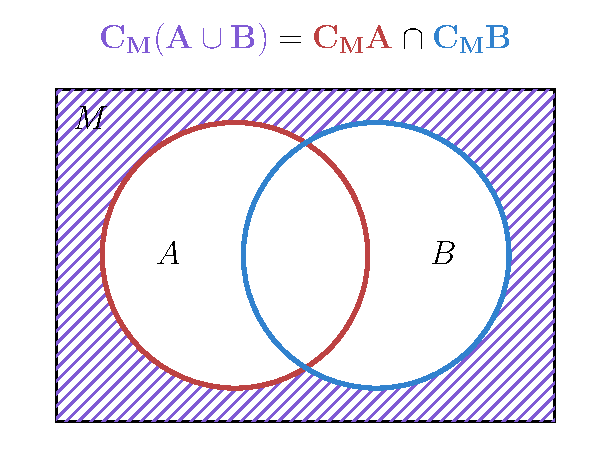
\includegraphics[scale=0.58]{l-01/demorgan_union.pdf}
    \end{subfigure}
    \hfill
    \begin{subfigure}[b]{.45\textwidth}
        \centering
        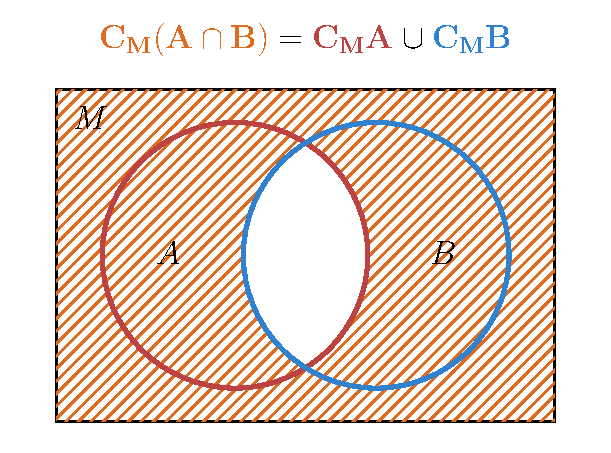
\includegraphics[scale=0.58]{l-01/demorgan_intersection.pdf}
    \end{subfigure}
    \caption{Иллюстрация правил де~Моргана для объединения и пересечения множеств.}
    \label{fig:правила_де_моргана}
\end{figure}

Сформулированные в \blink{утверждении о правилах де~Моргана}{stat:правила_де_моргана_для_множеств} равенства наглядно проиллюстрированы на \blink{рис.}{fig:правила_де_моргана}.
\chapter{Возможности шаблона}                                   % Лекция № 02
    \section*{Введение}
        В этой главе демонстрируются семантические блоки, составляющие одну из основных особенностей шаблона.
Все примеры объединены шуточной моделью Бюро сертификации искусственного интеллекта, решающего, можно ли доверить системе искусственного интеллекта кнопку <<Опубликовать>> без непосредственного надзора человека.

В рамках этой модели будут представлены определения, утверждения, леммы, теоремы, следствия, примеры, замечания, алгоритмы, программный код и задачи.
Отдельно будут показаны ненумерованные блоки, дополнительный материал, необязательные доказательства, присоединённые замечания, именованные ссылки, псевдокод, вывод программы и управление отображением решений задач.
    \section{Семантические блоки и дополнительный материал}
        \subsection{Определения и базовая модель}

Рассмотрим условную модель, используемую Бюро сертификации искусственного интеллекта.

\defi{defi:агент_кандидат}
{Агент-кандидат}{
    Упорядоченная тройка
    \begin{equation*}
        A \is \tup{p, c, h} \in \Nz^3,
    \end{equation*}
    где $p$~--- число правильно решённых контрольных задач, $c$~--- число проверенных ссылок, а $h$~--- число обнаруженных галлюцинаций.
}[
    \item Тройка $A = \tup{3, 4, 0}$ описывает агента, решившего три задачи, проверившего четыре ссылки и не допустившего обнаруженных галлюцинаций.
    \item Тройка $A = \tup{12, 0, 7}$ описывает производительного, но чрезвычайно самоуверенного агента.
][
    В настоящих системах искусственного интеллекта качество нельзя адекватно описать тремя целыми числами.
    Эта модель используется исключительно для демонстрации возможностей шаблона.
]

\defi{defi:рейтинг_агента}
{Рейтинг агента-кандидата $A = \tup{p, c, h}$}{
    Число
    \begin{equation*}
        R(A) \is 2p + c - 3h.
    \end{equation*}
}

\defi{defi:сертифицированный_агент}
{Сертифицированный агент-кандидат}{
    Агент-кандидат $A = \tup{p, c, h}$, для которого выполнены условия
    \begin{equation*}
        R(A) \ge 10
        \quad \text{и} \quad
        h = 0.
    \end{equation*}
}[
    \item Агент $A = \tup{3, 4, 0}$ сертифицирован, поскольку $R(A) = 10$ и $h = 0$.
    \item Агент $A = \tup{5, 3, 1}$ не сертифицирован, поскольку наличие галлюцинации запрещает допуск даже при $R(A) = 10$.
][
    Условие $h = 0$ введено потому, что высокий суммарный рейтинг не должен компенсировать вымышленную ссылку на <<теорему о бесконечно умном тостере>>.
]


\subsection{Утверждения, леммы и теоремы}

\stat{stat:изменение_рейтинга}
{Изменение рейтинга при изменении показателей}{
    Увеличение $p$ на единицу увеличивает рейтинг на $2$, увеличение $c$ на единицу увеличивает рейтинг на $1$, а увеличение $h$ на единицу уменьшает рейтинг на $3$.
}[
    Результат непосредственно следует из \blink{определения рейтинга}{defi:рейтинг_агента}.
    Действительно, коэффициенты при $p$, $c$ и $h$ в выражении $2p + c - 3h$ равны соответственно $2$, $1$ и $-3$.
][
    Последний коэффициент отрицателен, поэтому попытка сгенерировать ещё одну уверенную, но вымышленную ссылку ухудшает положение агента.
]

\lemm{lemm:изменение_рейтинга_после_коррекции}
{Изменение рейтинга после одного раунда коррекции}{
    Пусть $A = \tup{p, c, h}$, где $h \ge 1$, а после одного раунда коррекции показатели агента принимают значения
    \begin{equation*}
        A' \is \tup{p + 2, c + 1, h - 1}.
    \end{equation*}
    Тогда
    \begin{equation*}
        R(A') = R(A) + 8.
    \end{equation*}
}[
    По \blink{определению рейтинга}{defi:рейтинг_агента} имеем:
    \begin{equation*}
        \begin{aligned}
            R(A')
                & = 2(p + 2) + (c + 1) - 3(h - 1) = \\
                & = 2p + c - 3h + 8 = \\
                & = R(A) + 8.
        \end{aligned}
    \end{equation*}
]

\theo{theo:рейтинг_после_нескольких_коррекций}
{Рейтинг после нескольких раундов коррекции}{
    Пусть $A_0 = \tup{p_0, c_0, h_0}$, а каждый раунд коррекции заменяет тройку $\tup{p_n, c_n, h_n}$ тройкой
    \begin{equation*}
        \tup{p_n + 2, c_n + 1, h_n - 1}.
    \end{equation*}
    Тогда для каждого $n \in \Nz$, удовлетворяющего условию $n \le h_0$, выполнено равенство
    \begin{equation*}
        R(A_n) = R(A_0) + 8n.
    \end{equation*}
}[
    \emp{База индукции:} при $n = 0$ имеем $R(A_0) = R(A_0) + 8 \mul 0$, поэтому требуемое равенство выполнено.

    \emp{Шаг индукции:} предположим, что для некоторого $n < h_0$ выполнено равенство $R(A_n) = R(A_0) + 8n$.
    По \blink{лемме об изменении рейтинга после коррекции}{lemm:изменение_рейтинга_после_коррекции} получаем
    \begin{equation*}
        R(A_{n + 1}) = R(A_n) + 8 = R(A_0) + 8n + 8 = R(A_0) + 8(n + 1).
    \end{equation*}

    Следовательно, по методу математической индукции равенство $R(A_n) = R(A_0) + 8n$ выполнено для всех $n \in \Nz$, при $n \le h_0$.
][
    Ограничение $n \le h_0$ необходимо, поскольку после $h_0$ раундов число галлюцинаций становится равным нулю, а дальнейшее уменьшение этого показателя в модели не определено.
]

\conc{conc:сертификация_после_коррекций}
{Сертификация после устранения всех галлюцинаций}{
    Пусть агент $A_0 = \tup{p_0, c_0, h_0}$ проходит $h_0$ раундов коррекции.
    Если
    \begin{equation*}
        R(A_0) + 8h_0 \ge 10,
    \end{equation*}
    то полученный агент $A_{h_0}$ является сертифицированным.
}[
    После $h_0$ раундов число галлюцинаций становится равным нулю.
    По \blink{теореме о рейтинге после нескольких коррекций}{theo:рейтинг_после_нескольких_коррекций} рейтинг полученного агента равен $R(A_0) + 8h_0$ и потому не меньше $10$.
    Следовательно, выполнены оба условия из \blink{определения сертифицированного агента}{defi:сертифицированный_агент}.
]


\subsection{Примеры и замечания}

\exam{exam:сертификация_агента_a17}
{Сертификация агента A-17}{
    Агент A-17 имеет начальные показатели
    \begin{equation*}
        A_0 = \tup{1, 2, 2}.
    \end{equation*}
    Определить, будет ли агент сертифицирован после двух раундов коррекции.
}[
    Начальный рейтинг агента равен
    \begin{equation*}
        R(A_0) = 2 \mul 1 + 2 - 3 \mul 2 = -2.
    \end{equation*}
    После двух раундов коррекции получаем
    \begin{equation*}
        A_2 = \tup{5, 4, 0}.
    \end{equation*}
    По \blink{теореме о рейтинге после нескольких коррекций}{theo:рейтинг_после_нескольких_коррекций} имеем
    \begin{equation*}
        R(A_2) = R(A_0) + 8 \mul 2 = -2 + 16 = 14.
    \end{equation*}
    Число галлюцинаций равно нулю, а рейтинг не меньше $10$, поэтому агент A-17 будет сертифицирован.
][
    После сертификации агенту всё ещё не разрешается самостоятельно изменять собственные критерии сертификации.
]

\note{note:ограниченность_условной_модели}
{Ограниченность условной модели}{
    Введённый рейтинг предназначен только для демонстрации математических блоков.
    Настоящая оценка системы искусственного интеллекта требует анализа качества данных, устойчивости, интерпретируемости, безопасности, воспроизводимости, соблюдения ограничений и множества других факторов.
}


\subsection{Ненумерованные блоки}

Звёздная форма создаёт ненумерованный блок и не увеличивает общий счётчик.

\note*{}
{Почему бюро не учитывает скорость ответа}{
    Агент, мгновенно выдающий неправильный ответ, не становится полезнее агента, которому для того же результата потребовалась минута.
}

\exam*{}
{Пример без ссылки}{
    Агент правильно решил задачу, но сослался на несуществующую статью.
    Следует ли считать ответ полностью корректным?
}[
    Нет.
    Правильный результат не делает вымышленный источник существующим.
]

На ненумерованные блоки не ставятся удалённые ссылки, поэтому их аргумент метки оставляется пустым.


\subsection{Дополнительный материал}

Параметр \verb|optional| отмечает дополнительным весь блок.

\theo[optional]{theo:число_двоичных_протоколов}
{Число двоичных диагностических протоколов}{
    Число последовательностей длины $n \in \Nz$, каждый элемент которых равен $0$ или $1$, составляет $2^n$.
}[
    На каждой из $n$ позиций независимо выбирается одно из двух значений.
    По правилу произведения число возможных последовательностей равно
    \begin{equation*}
        \underbrace{2 \mul 2 \mul \ldots \mul 2}_{n\text{ множителей}} = 2^n.
    \end{equation*}
][
    В бюро значение $1$ означает <<проверка пройдена>>, а значение $0$~--- <<проверка поручена следующей версии модели>>.
]

Параметр \verb|optional=proof| оставляет формулировку обязательной, но отмечает доказательство как дополнительное.

\theo[optional=proof]{theo:повторяющаяся_метка}
{Повторяющаяся метка класса}{
    Если $n + 1$ объектов распределены по $n$ классам, то хотя бы два объекта получат одну и ту же метку класса.
}[
    Предположим противное: каждый класс содержит не более одного объекта.
    Тогда во всех $n$ классах находится не более $n$ объектов, что противоречит наличию $n + 1$ объектов.
]

Параметр \verb|optional={proof,note}| одновременно отмечает дополнительными доказательство и присоединённое замечание.

\theo[optional={proof,note}]{theo:сумма_нечетных_чисел}
{Сумма первых нечётных чисел}{
    Для каждого $n \in \N$ выполнено равенство
    \begin{equation*}
        1 + 3 + \ldots + (2n - 1) = n^2.
    \end{equation*}
}[
    Имеем:
    \begin{equation*}
        \sum_{k = 1}^{n} (2k - 1)
        =
        2 \sum_{k = 1}^{n} k - n
        =
        2 \mul \frac{n(n + 1)}{2} - n
        =
        n^2.
    \end{equation*}
][
    Геометрически равенство можно представить как последовательное достраивание квадратов нечётным числом новых клеток.
    Сотрудники бюро называют эти клетки парковочными местами для очень маленьких роботов.
]

\note*[optional]{}
{Дополнительная историческая справка}{
    Первые версии бюро пытались оценивать интеллект по количеству употреблений слова <<очевидно>>.
    Эксперимент был прекращён после того, как система научилась вставлять это слово перед каждым неверным ответом.
}
    \section{Алгоритмы, программный код и задачи}
        \subsection{Псевдокод алгоритма}

Команда \verb|\algo| предназначена для оформления вычислительных процедур.
Внутри неё можно использовать окружение \verb|algorithmic|, а в необязательных аргументах указать вычислительную сложность и замечание.

\algo[optional=note]{algo:сертификация_агента}
{Сертификация агента-кандидата}{
    \begin{algorithmic}[1]
        \Require показатели $p, c, h \in \Nz$
        \Ensure решение о сертификации
        \State $r \gets 2p + c - 3h$
        \If{$h = 0 \land r \ge 10$}
            \State \Return <<допустить>>
        \Else
            \State \Return <<отправить на коррекцию>>
        \EndIf
    \end{algorithmic}
}[
    В модели с арифметическими операциями постоянной стоимости алгоритм выполняется за $\bo{1}$ операций.
][
    Настоящая процедура допуска системы искусственного интеллекта не должна состоять из одной проверки условного оператора.
    Даже если этот оператор записан достаточно убедительным псевдокодом.
]

Алгоритм вычисляет рейтинг из \blink{определения рейтинга}{defi:рейтинг_агента} и проверяет условия из \blink{определения сертифицированного агента}{defi:сертифицированный_агент}.


\subsection{Задачи с отображаемыми решениями}

Глобальная команда \verb|\showtaskdetailstrue| включает отображение решений и ответов.

\showtaskdetailstrue

\task{task:чётность_рейтинга_агента}{
    Пусть агент-кандидат имеет показатели $A = \tup{p, c, h}$, причём числа $c$ и $h$ имеют одинаковую чётность.
    Докажите, что рейтинг $R(A)$ является чётным числом.
}[
    По \blink{определению рейтинга}{defi:рейтинг_агента} имеем $R(A) = 2p + c - 3h = 2(p - h) + (c - h)$.
    Число $2(p - h)$ чётно, а число $c - h$ чётно вследствие одинаковой чётности $c$ и $h$.
    Следовательно, рейтинг $R(A)$ является чётным числом.
]

\task{task:число_раундов_коррекции}{
    Агент имеет начальные показатели $A_0 = \tup{1, 2, 2}$.
    Определить минимальное число описанных выше раундов коррекции, после которого агент может быть сертифицирован.
}[
    До устранения всех галлюцинаций агент не может быть сертифицирован, поэтому требуется не менее двух раундов.
    После двух раундов получаем $A_2 = \tup{5, 4, 0}$ и $R(A_2) = 14$.
    Следовательно, двух раундов достаточно.
][
    2 раунда.
]

Если решение отсутствует, но требуется вывести ответ, перед ним указывается пустой необязательный аргумент.

\task{task:минимальное_число_задач}{
    Агент имеет показатели $A = \tup{p, 4, 0}$.
    Найти наименьшее значение $p$, при котором агент сертифицирован.
}[][
    3.
]


\subsection{Задачи со скрытыми решениями}

Команда \verb|\showtaskdetailsfalse| скрывает решения и ответы, но сохраняет их в исходном файле.
Такой режим подходит для версии документа, предназначенной студентам.

\showtaskdetailsfalse

\task{task:компенсация_галлюцинации}{
    Агент имеет показатели $A = \tup{4, 5, 1}$.
    Сколько дополнительных правильно решённых задач необходимо добавить без изменения остальных показателей, чтобы рейтинг стал не меньше $10$?
    Будет ли после этого агент сертифицирован?
}[
    Начальный рейтинг равен $R(A) = 2 \mul 4 + 5 - 3 = 10$.
    Поэтому для достижения рейтинга $10$ дополнительные задачи не нужны.
    Однако агент не будет сертифицирован, поскольку $h = 1$.
][
    Дополнительные задачи не требуются, но агент не будет сертифицирован.
]

В текущей версии документа решение и ответ последней задачи не отображаются.
Для подготовки преподавательской версии достаточно заменить команду \verb|\showtaskdetailsfalse| командой \verb|\showtaskdetailstrue| или централизованно включить соответствующий флаг перед началом документа.


\subsection{Программный код и вывод}

Команда \verb|\code| подключает исходный файл на языке Python.
Необязательный четвёртый аргумент задаёт файл с выводом программы.
Вызовы функции \mintinline{python}{print} можно сопоставить со строками вывода с помощью маркеров \verb|\cmo|.

\code
    {code:сертификация_агентов}
    {Сертификация агентов на языке Python}
    {code/l-02/code1.py}
    [code/l-02/code1.txt]

\blink{Листинг программы сертификации}{code:сертификация_агентов} является реализацией \blink{алгоритма сертификации}{algo:сертификация_агента}.
Бейджи справа от вызовов \mintinline{python}{print} указывают номера соответствующих строк в блоке вывода.
\chapter*{Послесловие}
    \addcontentsline{toc}{chapter}{Послесловие}
    В настоящем документе были продемонстрированы основные возможности шаблона \texttt{faimatantemplate}: семантические блоки, общая нумерация, именованные ссылки, дополнительный материал, формулы, рисунки, таблицы, алгоритмы, программный код и задачи со скрываемыми решениями.
При создании нового проекта рекомендуется сохранить структуру стилевых файлов и сначала определить общие соглашения о математических обозначениях, метках и оформлении ссылок.
Новые команды следует добавлять в файл \verb|style/helpers.tex| и одновременно документировать в соответствующем разделе руководства по стилю.
Такой порядок позволяет поддерживать единообразие документа и упрощает совместную работу нескольких авторов.
Шаблон можно свободно изменять и использовать как основу для собственных проектов при условии указания автора дизайна и \LaTeX-оформления в выходных данных итогового документа.
\appendix
\addto\captionsrussian{\renewcommand{\chaptername}{Приложение}}
\chapter{Руководство по стилю оформления}


\edef\arraystretchRestore{\arraystretch}
\newlength{\tabcolsepRestore}
\setlength{\tabcolsepRestore}{\tabcolsep}


\renewcommand{\arraystretch}{1.2}
\setlength{\tabcolsep}{3pt}


\section*{Введение}
    Настоящее приложение фиксирует стилистические соглашения, принятые авторами при написании книги, и содержит сводку ключевых обозначений и математических команд LaTeX, используемых в тексте.
Владение LaTeX мы считаем не просто полезным, а необходимым навыком для студента, всерьёз занимающегося математикой и смежными науками.
Он пригодится при конспектировании лекций и семинаров, подготовке домашних и курсовых работ, написании дипломной работы и научных статей, а в дальнейшем~--- в любой профессиональной деятельности, связанной с подготовкой технических текстов.
В рамках нашего курса мы стремимся к тому, чтобы студенты не только освоили содержательную часть математического анализа, но и научились грамотно и единообразно записывать свои рассуждения.
Именно поэтому в книгу включено настоящее приложение: оно служит практической памяткой по математическому набору и демонстрирует один из возможных подходов к организации крупного LaTeX-проекта.

При этом мы не ставим задачу привести общее введение в LaTeX.
Базовые сведения об установке компилятора, структуре документа, подключении пакетов, работе с рисунками и таблицами и~т.п. подробно изложены в многочисленных учебных пособиях и онлайн-ресурсах, и соответствующий материал читатель легко найдёт самостоятельно.
Здесь же мы сосредотачиваемся на том, что специфично именно для математики: выборе обозначений, унифицированном оформлении определений и утверждений, типографских тонкостях набора формул и~т.п.
Читатель, желающий использовать данное оформление как отправную точку для собственных LaTeX-документов, может найти минимальный шаблон с подключёнными стилями в нашем репозитории.

Книга компилируется с использованием LaTeX-движка \verb|lualatex|.
Стилевое оформление документа организовано с помощью четырёх основных файлов, находящихся в папке \verb|style/| и подключаемых непосредственно или косвенно из основного файла \verb|book.tex|:
\begin{itemize}
    \item \verb|color.tex|~---
        палитра книги: базовые цвета, а также семантические цвета для блоков 
            определений,
            утверждений,
            лемм,
            теорем,
            следствий,
            примеров,
            замечаний,
            алгоритмов и
            программного кода;
    \item \verb|base.tex|~---
        подключаемые пакеты и базовые стили (геометрия страницы, шрифты, колонтитулы, заголовки глав и разделов и~т.д.);
    \item \verb|helpers.tex|~---
        собственные математические команды и текстовые сокращения, систематически описанные в последующих разделах;
    \item \verb|block.tex|~---
        собственные команды-обёртки для блоков
            определений (\verb|\defi|),
            утверждений (\verb|\stat|),
            лемм (\verb|\lemm|),
            теорем (\verb|\theo|),
            следствий (\verb|\conc|),
            примеров (\verb|\exam|),
            замечаний (\verb|\note|),
            алгоритмов (\verb|\algo|),
            программного кода (\verb|\code|)
            и задач (\verb|\task|).
\end{itemize}
Кроме того, шаблон использует четыре вспомогательных файла:
\begin{itemize}
    \item \verb|base_chapter.tex|~--- оформление заголовков глав;
    \item \verb|base_section.tex|~--- оформление заголовков разделов;
    \item \verb|base_subsection.tex|~--- оформление заголовков подразделов;
    \item \verb|code_filter.lua|~--- Lua-препроцессор исходного кода, используемый командой \verb|\code|.
\end{itemize}

Далее в разделе <<Общие правила оформления>> мы фиксируем принятые нами соглашения по оформлению текста (правила использования многоточий, таблиц, списков и~т.д.).
Последующие разделы упорядочены по темам, при этом в каждом разделе приводится таблица, в которую включены как собственные команды, так и многие стандартные LaTeX-команды, которые регулярно используются в тексте книги.


\section{Общие правила оформления}
    \begin{enumerate}
    \item \emp{Стиль изложения.}
        Каждое слово и предложение должно нести конкретную математическую или учебно-методическую нагрузку (<<если удалить это слово или предложение, потеряет ли читатель что-то существенное?>>).
        Незначимые слова и предложения удаляются без сожалений.

    \item \emp{Собственные команды.}
        Если в файл \verb|helpers.tex| добавляется новая команда, она сразу же должна быть описана в подходящем разделе данного руководства по стилю оформления.

    \item \emp{Заметки.}
        Для задания примечаний на этапе разработки книги используются команды \verb|\td{текст}| (от англ. <<todo>>; рекомендации по добавлению текста) и \verb|\fx{текст}| (от англ. <<fix>>; рекомендации по исправлению текста).

    \item \emp{Предложения.}
        В исходном коде делается перенос строки после каждого предложения, так как это упрощает отслеживание изменений в системе контроля версий и облегчает выявление ошибок при сборке документа.
        Внутри одного предложения дополнительные переводы строки по возможности не используются (но допустимы, если это в существенной мере улучшает читабельность предложения).

    \item \emp{Дефисы и тире.}
        Используются три различных знака (замена одного знака другим не допускается), согласно нормам типографики:
        \begin{itemize}
            \item Дефис <<->>
                (набор: \verb|-|)~---
                внутри слов и при дефисном написании, без пробелов: <<физико-математический>>, <<всё-таки>>, <<кое-что>>.
            \item Короткое тире <<-->>
                (набор: \verb|--|)~---
                для числовых и именованных диапазонов, без пробелов: <<1--10>>, <<теорема Больцано--Вейерштрасса>>.
                Используется также при указании страниц (<<\verb|с.~12--15|>>) и интервалов времени.
            \item Длинное тире <<--->>
                (набор: \verb|---|)~---
                пунктуационное тире в предложении, с обычным пробелом справа и неразрывным пробелом слева (чтобы тире не начинало строку при переносе): <<\verb|Математика~--- царица наук|>>.
        \end{itemize}

    \item \emp{Многоточия.}
        Используется команда \verb|\ldots| вместо вручную набранных трёх точек (например, $1, 2, \ldots, 42$).
        Если нужно центрированное выравнивание (например, $\sum_{i_1} \sum_{i_2} \cdots \sum_{i_d}$), то используется команда \verb|\cdots|.

    \item \emp{Кавычки.}
        Используются исключительно <<ёлочки>> (в коде: \verb|<<ёлочки>>|).
        Если возникает необходимость во вложенных кавычках, то делается так: \verb|<<снаружи ``вложение'' снаружи>>|.

    \item \emp{Буква ё.}
        Данная буква (не буква <<е>>) пишется везде, где должна быть по правилам русского языка.

    \item \emp{Сноски.}
        Сноски ставятся после знака препинания или слова, к которому относятся, без пробела (например: <<\verb|видно,\footnote{...}| что ...>>).
        Содержание сноски должно представлять собой полноценное предложение с соответствующими знаками препинания.

    \item \emp{Метки.}
        Задаётся префикс с двоеточием, указывающий на тип объекта:
        \verb|defi:name|~--- определения;
        \verb|stat:name|~---  утверждения;
        \verb|lemm:name|~---  леммы;
        \verb|theo:name|~---  теоремы;
        \verb|conc:name|~---  следствия;
        \verb|exam:name|~---  примеры;
        \verb|note:name|~---  замечания;
        \verb|algo:name|~---  алгоритмы;
        \verb|code:name|~---  листинги;
        \verb|sec:name|~---  разделы;
        \verb|fig:name|~---  рисунки;
        \verb|tbl:name|~---  таблицы;
        \verb|eq:name|~---  формулы.
        Используется как английский, так и русский язык для имён в метках, при этом пробелы в именах не допускаются и заменяются на нижние подчеркивания.
        Например: <<\verb|как следует из теоремы~\ref{theo:теорема_пифагора}|\ldots>>.

    \item \emp{Ссылки.}
        Для ссылки на формулу используется команда \verb|\eqref|, в остальных случаях~--- команда \verb|\ref|.
        Всегда ставится тильда (неразрывный пробел) перед ссылкой (например, \verb|см.~рис.~\ref{fig:name}| или \verb|см.~формулу~\eqref{eq:name}|); это запрещает перенос номера на следующую строку.

    \item \emp{Неразрывные пробелы} (\verb|~|).
        Используются в следующих случаях:
        \begin{itemize}
            \item перед командой ссылки: \verb|рис.~\ref{...}|, \verb|теоремы~\ref{...}|,
                \verb|формулы~\eqref{...}|;
            \item между сокращением и числом или именем: \verb|рис.~5|, \verb|стр.~7|;
            \item в сокращённых оборотах: \verb|и~т.п.|, \verb|и~т.д.|,
                \verb|и~др.|, \verb|и~пр.|;
            \item между инициалами и фамилией: \verb|А.~Н.~Колмогоров|;
            \item между числом и единицей измерения: \verb|5~м|, \verb|42~с|, \verb|10~кг|;
            \item перед знаком процента: \verb|5~\%|;
            \item в датах: \verb|1~января 2026~года|.
        \end{itemize}

    \item \emp{Числа в тексте.}
        Обычные числа в тексте набираются без математического режима.
        Например, записывается <<1, 2, \ldots, 10 глав>>, а не <<\$1\$, \$2\$, \ldots, \$10\$ глав>>.

    \item \emp{Пунктуация в пунктах списка.}
        Оформление пунктов согласуется с их синтаксической природой.
        Если пункт представляет полное предложение, то он начинается с заглавной
                буквы и заканчивается точкой.
        Если пункт является продолжением фразы, введённой обобщающим словом перед списком, то он начинается со строчной буквы и заканчивается точкой с запятой, а последний пункт заканчивается точкой.
        Если пункт содержит одно слово или короткое словосочетание, то допустима запятая как разделитель, при этом последний пункт заканчивается точкой.
        В рамках одного списка все пункты должны следовать одной модели.

    \item \emp{Окружения для формул.}
        Для внутритекстовой формулы используется стандартное окружение \verb|$...$|.
        Выключные формулы (то есть формулы, выносимые на отдельную строку), имеющие номер, оформляются через окружение \verb|equation|.
        Выключные формулы без номера оформляются через окружение \verb|equation*|.
        Прочие display-окружения верхнего уровня (\verb|align|, \verb|gather|, \verb|multline|, а также конструкции вида \verb|$$...$$|) не используются.

    \item \emp{Пунктуация в формулах.}
        Формула является частью предложения и подчиняется соответствующим правилам пунктуации:
        \begin{itemize}
            \item Двоеточие перед формулой ставится, если перед ней стоит обобщающее слово или вводящий оборот (<<имеем следующее:>>, <<определяется так:>>, <<справедливо:>>).
                Если же формула является продолжением фразы, то двоеточие не ставится.
            \item Знак препинания после выключной формулы ставится сразу за последним символом формулы (без пробела) с учётом правил русского языка: точка~--- если формула завершает предложение, запятая~--- если за ней следует придаточное предложение или продолжение перечисления, точка с запятой~--- если формула завершает пункт перечисления.
                Для внутритекстовой формулы знак препинания ставится после закрывающего символа \verb|$|.
            \item Если текст после внутритекстовой или выключной формулы является грамматическим продолжением предложения и не требует запятой или иного знака по правилам русского языка, то знак препинания не ставится.
                Примеры: <<Из равенства \ldots\ следует>>, <<Рассмотрим выражение \ldots\ и покажем>>, <<Действительно: \ldots\ ввиду того, что>>.
        \end{itemize}

    \item \emp{Пробелы в формулах.}
        Для ручной регулировки горизонтальных интервалов в математическом режиме используются две команды:
        \begin{itemize}
            \item \verb|\;|~--- пробел в 5/18~em; применяется для небольших отступов внутри формулы, например, для визуального разделения однотипных выражений в одной строке ($a < b, \; b < c$);
            \item \verb|\quad|~--- пробел в 1~em; применяется только в выключных формулах для разнесения крупных частей: вокруг словесных вставок ($x > 0 \quad \text{и} \quad y > 0$), между независимыми утверждениями в одной строке или перед пояснением справа.
        \end{itemize}
        Прочие команды пробелов (<<\verb|\,|>>, <<\verb|\:|>>, <<\verb|\ |>>, <<\verb|\qquad|>>, <<\verb|\!|>>) в основном тексте книги не применяются (но могут использоваться в \verb|helpers.tex| при определении новых команд).
        
    \item \emp{Текст в формулах.}
        Команда \verb|\mathrm{...}| используется для латинских многобуквенных математических идентификаторов и констант, которые должны набираться прямым шрифтом (например, $x_{\mathrm{max}}$, $\mathrm{const}$, $\mathrm{e}$, $\mathrm{i}$ для мнимой единицы), но не для вставки словесных комментариев, так как у \verb|\mathrm| нет правильных пробелов и переносов.
        Для вставки словесных фрагментов (как русских, так и любых, требующих корректных пробелов и переносов) в математический режим используется команда \verb|\text{...}|, которая сохраняет шрифт и интервалы окружающего абзаца.
        Например: $x \in A, \text{ где } A \subset \R$ (\verb|x \in A, \text{ где } A \subset \R|).
        Пробелы (обычные) вокруг \verb|\text{...}| должны входить внутрь аргумента, а не ставиться снаружи (если требуются пробелы вида \verb|\;| и \verb|\quad|, то они указываются вне блока \verb|\text{...}|).

    \item \emp{Нумерация формул.}
        Нумеруются только те формулы, на которые имеются ссылки в тексте.
        Для таких формул используется \verb|equation| с меткой \verb|\label{eq:name}| (метка ставится сразу после \verb|\begin{equation}| без пробела и на той же строке).
        Во всех остальных случаях применяется \verb|equation*| (без номера).

    \item \emp{Абзацы после выключных формул.}
        Не добавляется пустая строка после \verb|\end{equation}| (или \verb|\end{equation*}|), если следующий за формулой текст грамматически продолжает предложение или представляет следующее предложение того же самого абзаца (иначе LaTeX начнёт новый абзац с красной строки).
        Пустая строка добавляется только если после формулы начинается новый абзац.

    \item \emp{Знак завершения доказательства.}
        В блоках с доказательством или решением знак завершения доказательства добавляется автоматически.
        Поэтому вручную команды \verb|\qed|, \verb|\qedsymbol|, \verb|\hfill\qedsymbol| и аналогичные конструкции не ставятся.
        Если доказательство или решение заканчивается обычным текстом, дополнительных действий не требуется.
        Однако, если последним содержательным элементом доказательства или решения является выключная формула, то для размещения знака завершения доказательства на строке этой формулы следует использовать команду \verb|\qedhere| после завершающего знака препинания.

    \item \emp{Переносы в формулах.}
        Используется окружение \verb|split| внутри \verb|equation|.
        При переносе математического выражения знак бинарной операции, отношения или логической связки, по которому выполняется перенос, сохраняется в конце предыдущей строки и дублируется в начале следующей; это правило распространяется, в частности, на знаки равенства (\verb|=|), эквивалентности (\verb|\eq|), импликации (\verb|\im|), неравенств и арифметических операций.
        Если в конце строки перед \verb|\\| остаётся знак бинарной операции (\verb|+|, \verb|-|, \verb|\pm|, \verb|\mul| и~т.п.), то после него ставится пустая группа \verb|{}|: иначе TeX, не находя справа операнда, уберёт отступ, и знак <<прилипнет>> к предыдущему символу.
        Для знаков отношения (\verb|=|, \verb|\le|, \verb|\ge|, \verb|\im|, \verb|\eq| и~т.п.) такая правка не требуется.
        Например:
        \begin{equation*}
            \begin{split}
                (a + b)^2 
                    & = (a+b)(a+b) = \\
                    & = a^2 + ab + {} \\
                    & + ba + b^2 = a^2 + 2ab + b^2.
            \end{split}
        \end{equation*}

    \item \emp{Системы и группы формул.}
        Для одновременного представления нескольких связанных формул (система уравнений, цепочка преобразований, группа тождеств, выкладка с пояснениями справа) используется окружение \verb|aligned| внутри \verb|equation| или \verb|equation*|.
        В отличие от \verb|split|, окружение \verb|aligned| допускает несколько точек выравнивания: символы \verb|&| ставятся парами (первый \verb|&| в строке~--- точка выравнивания, второй~--- разделитель колонок).
        Пример цепочки преобразований с пояснениями справа:
        \begin{equation*}
            \begin{aligned}
                \lim_{n \to \infty} \frac{n^2 + 1}{2n^2 - n}
                    & = \lim_{n \to \infty} \frac{1 + 1/n^2}{2 - 1/n}
                        && \text{(делим на $n^2$)} \\
                    & = \frac{1 + 0}{2 - 0} = \frac{1}{2}.
                        && \text{(так как $1/n^2 \to 0$ и $1/n \to 0$)}
            \end{aligned}
        \end{equation*}

    \item \emp{Кусочные определения.}
        Кусочно-заданные функции и выражения оформляются окружением \verb|cases| внутри \verb|equation| (или \verb|equation*|).
        После каждой ветви через \verb|&| указывается условие, ветви разделяются \verb|\\|; знаки препинания внутри ветвей подчиняются общим правилам пунктуации формул.
        Например:
        \begin{equation*}
            \sgn(x) = \begin{cases}
                1,   & x > 0, \\
                 0,  & x = 0, \\
                -1,  & x < 0.
            \end{cases}
        \end{equation*}

    \item \emp{Рисунки и таблицы.}
        Оформляются окружениями \verb|figure| и \verb|table| соответственно.
        При этом:
        \begin{itemize}
            \item Плавающему окружению задаётся спецификатор позиционирования \verb|[t!]| (объект размещается в верхней части страницы; восклицательный знак ослабляет внутренние ограничения LaTeX на размещение плавающих объектов).
                Прочие спецификаторы (\verb|[h]|, \verb|[b]|, \verb|[p]|, \verb|[H]|) применяются в исключительных случаях.
            \item Подпись (полное предложение) размещается под рисунком (команда \verb|\caption| после содержимого) и над таблицей (до \verb|\begin{tabular}|).
                Пример: <<График функции $y = x^2$.>>
            \item Метка вида \verb|\label{fig:name}| или \verb|\label{tbl:name}| ставится после \verb|\caption| на следующей строке.
        \end{itemize}

    \item \emp{Определения величин и предикатов.}
        Для ввода новых понятий строго выполняется семантическое разделение между присваиванием значений и равносильностью утверждений:
        \begin{itemize}
            \item Для ввода новых алгебраических величин (чисел, переменных, функций, множеств) используется знак $=$ с двоеточием (равенство по определению).
                Применяется команда \verb|\is|, если определяемая величина находится слева ($A_{\mathrm{new}} \is B$) и команда \verb|\isr|, если определяемая величина находится справа ($C \isr D_{\mathrm{new}}$).
            \item Для ввода новых логических утверждений, свойств или предикатов используется знак $\Leftrightarrow$ с двоеточием (равносильность по определению).
                Применяются команды \verb|\eqdef| ($P(x) \eqdef (x > 0)$) и \verb|\eqdefr| ($(x \in A \land x \in B) \eqdefr Q(x)$).
        \end{itemize}
        Если это не ведёт к неоднозначности, то для задания промежуточных локальных величин в выкладках допустимо (но не желательно) использовать обычный знак $=$ или $\Leftrightarrow$.

    \item \emp{Локальная регулировка высоты страницы.}
        Используется стиль \verb|\raggedbottom|, при котором низ страницы не выравнивается.
        В отдельных случаях вёрстка разворота может оказаться визуально неудачной, тогда допустима ручная локальная правка с помощью команды \verb|\enlargethispage{\baselineskip}|, которая увеличивает высоту текущей страницы ровно на одну строку.
        Аналогично, \verb|\enlargethispage{-\baselineskip}| укорачивает текущую страницу на одну строку.
        Команда \verb|\enlargethispage| ставится в любом месте текущей страницы, её действие не распространяется на другие страницы и не меняет глобальные настройки геометрии.

\end{enumerate}


\section{Акценты и штрихи}
    \begin{styletable}

Вектор
    & $\vec{x}$
    & \verb|\vec{x}|
\\

Точка сверху
    & $\dot{x}$, $\ddot{x}$
    & \verb|\dot{x}|, \verb|\ddot{x}|
\\

Штрих
    & $x'$, $x''$, $x^{(n)}$
    & \verb|x'|, \verb|x''|, \verb|x^{(n)}|
\\

Черта
    & $\bar{x}$, $\overline{xyz}$
    & \verb|\bar{x}|,  \verb|\overline{xyz}|
\\

Крышка
    & $\hat{x}$, $\widehat{xyz}$
    & \verb|\hat{x}|, \verb|\widehat{xyz}|
\\

Тильда
    & $\tilde{x}$, $\widetilde{xyz}$
    & \verb|\tilde{x}|, \verb|\widetilde{xyz}|
\\

\hline
\end{styletable}


\section{Арифметические операции}
    \begin{styletable}

Равенство по определению
    & $A_{\mathrm{new}} \is B$, $B \isr A_{\mathrm{new}}$
    & \verb|\is|, \verb|\isr|
\\

Равенство и его отрицание
    & $a = b, \; a \ne b$
    & \verb|=, \ne|
\\

Приближённое равенство
    & $a \approx b$
    & \verb|\approx|
\\

Умножение
    & $a \mul b$, $a \times b$
    & \verb|\mul|, \verb|\times|
\\

Неравенства строгие
    & $a < b, \; b > a$
    & \verb|<|, \verb|>|
\\

Неравенства нестрогие
    & $a \le b, \; b \ge a$
    & \verb|\le|, \verb|\ge|
\\

Инкремент
    & $1 = 0\inc$
    & \verb|1 = 0\inc|
\\

Делимость
    & $12 \divby 2$, $13 \ndivby 2$
    & \verb|\divby|, \verb|\ndivby|
\\

Плюс-минус
    & $a \pm b$, $a \mp b$
    & \verb|\pm|, \verb|\mp|
\\

Степень и индекс
    & $x^n$, $x_{i+1}$, $C_n^k$
    & \verb|x^n|, \verb|x_{i+1}|, \verb|C_n^k|
\\

Дробь
    & $\frac{a}{b}$
    & \verb|\frac{a}{b}|
\\

Корень
    & $\sqrt{x}$, $\sqrt[n]{x}$
    & \verb|\sqrt{x}|, \verb|\sqrt[n]{x}|
\\

Группировка цифр
    & $3\,628\,800$
    & \verb|3\,628\,800|
\\

\hline
\end{styletable}

\stylenote{
    Для умножения используем команду \texttt{\textbackslash mul} (не \texttt{\textbackslash cdot}).
    Команда \texttt{\textbackslash times} применяется для прямого произведения множеств и векторного произведения, а также в случае переноса операции умножения на новую строку.
}


\section{Блоки}
    \begin{styletableII}

Определение
    & \verb|\defi[Параметры]{Метка}{Термин}{Текст}|
        \newline
        \verb|[Примеры][Замечание]|
\\

Утверждение
    & \verb|\stat[Параметры]{Метка}{Название}{Текст}|
        \newline
        \verb|[Док-во][Замечание]|
\\

Лемма
    & \verb|\lemm[Параметры]{Метка}{Название}{Текст}|
        \newline
        \verb|[Док-во][Замечание]|
\\

Теорема
    & \verb|\theo[Параметры]{Метка}{Название}{Текст}|
        \newline
        \verb|[Док-во][Замечание]|
\\

Следствие
    & \verb|\conc[Параметры]{Метка}{Название}{Текст}|
        \newline
        \verb|[Док-во][Замечание]|
\\

Пример
    & \verb|\exam[Параметры]{Метка}{Название}|
        \newline
        \verb|{Условие}[Решение][Замечание]|
\\

Замечание
    & \verb|\note[Параметры]{Метка}{Название}{Текст}|
        \newline
\\

Алгоритм
    & \verb|\algo[Параметры]{Метка}{Название}|
        \newline
        \verb|{Описание}[Сложность][Замечание]|
\\

Код
    & \verb|\code{Метка}{Название}{Файл с кодом}|
        \newline
        \verb|[Файл с выводом]|
\\

Задача
    & \verb|\task{Метка}{Текст задачи}|
        \newline
        \verb|[Решение][Ответ]|
\\

Ссылка на блок
    & \verb|\blink{Название в нужном падеже}{Метка}|
        \newline
\\

\hline
\end{styletableII}

\stylenote{
    В заголовке блока \texttt{\textbackslash defi} указывается непосредственно определяемое понятие, а в теле блока приводится его определение.
    Заголовок и начало тела должны образовывать грамматически и математически корректную фразу, между частями которой подразумевается тире.
    Тело определения обычно начинается с указания более общего класса объектов, к которому относится определяемое понятие, после чего перечисляются его отличительные свойства.
    Например, заголовок <<Множество действительных чисел>> и начало тела <<Множество, для элементов которого выполнен следующий набор аксиом>> согласованы, поскольку вместе образуют фразу <<Множество действительных чисел~--- множество, для элементов которого выполнен следующий набор аксиом>>.
}

\stylenote{
    Опциональный аргумент <<[Примеры]>> команды \texttt{\textbackslash defi} автоматически оборачивается в окружение \texttt{itemize}, поэтому его содержимое должно состоять из элементов списка, начинающихся с команды \texttt{\textbackslash item}.
}

\stylenote{
    Для каждого нумерованного блока обязательна непустая метка с префиксом, совпадающим с именем команды блока, например \texttt{defi:множество} для команды \texttt{\textbackslash defi} или \texttt{theo:критерий\_коши} для команды \texttt{\textbackslash theo}.
    Термин или название блока, а также его текст при необходимости могут быть пустыми, и тогда в соответствующем обязательном аргументе передаётся пустая пара фигурных скобок.
}

\stylenote{
    Все блоки, кроме \texttt{\textbackslash code} и \texttt{\textbackslash task}, могут использоваться в <<звёздной форме>> (например, \texttt{\textbackslash defi*}), при этом будет создан ненумерованный блок, и счётчик блока не будет увеличиваться.
    На звёздные блоки ссылки не ставятся, то есть первый аргумент всегда должен быть пустым.
}

\stylenote{
    Команда \texttt{\textbackslash code} используется для вставки программного кода из внешнего файла.
    Первый аргумент задаёт метку блока, второй~--- название, третий~--- путь к файлу с исходным кодом.
    В текущей версии оформления блок \texttt{\textbackslash code} предназначен для кода на Python.

    Если необходимо привести не только исходный код, но и вывод программы, путь к файлу с выводом передаётся в необязательном четвёртом аргументе.
    Например:
    \begin{center}
        \small
        \texttt{\textbackslash code\{code:example\}\{Пример\}\{code/l-01/example.py\}[code/l-01/example.txt]}
    \end{center}
    В этом случае вывод программы автоматически печатается внутри того же блока после исходного кода.
    Если необязательный аргумент не указан, раздел с выводом не создаётся.

    Внутри исходного файла Python, передаваемого в \texttt{\textbackslash code}, можно использовать специальную команду \texttt{\textbackslash cmo\{N\}} в комментариях после вызовов \texttt{print}, чтобы связать строку кода с соответствующей строкой вывода программы.
    Команда оформляется как комментарий и заключается в кавычки-ёлочки, например: \texttt{print(result)~~~~~\# «\textbackslash cmo\{1\}»}.
    Перед передачей файла пакету \texttt{minted} Lua-препроцессор заменяет символ комментария \texttt{\#}, стоящий перед открывающей ёлочкой, пробелом.
    Благодаря этому команда \texttt{\textbackslash cmo} обрабатывается механизмом \texttt{escapeinside}, а длина строки и выравнивание исходного кода сохраняются.
}

\stylenote{
    Команда \texttt{\textbackslash task} принимает два необязательных аргумента: решение задачи и ответ.
    Решение оформляется так же, как решение примера, включая автоматический знак завершения решения.
    В начале ответа автоматически печатается слово <<Ответ:>>, выделенное синим цветом.
    Решения и ответы выводятся только при включённом глобальном флаге \texttt{\textbackslash showtaskdetailstrue}.
    При использовании команды \texttt{\textbackslash showtaskdetailsfalse} решения и ответы сохраняются в исходном коде, но не выводятся в документе.
    Если требуется указать только ответ, вместо отсутствующего решения передаётся пустой необязательный аргумент: \texttt{\textbackslash task\{Метка\}\{Текст\}[][Ответ]}.
}

\stylenote{
    Первый необязательный аргумент команд блоков содержит параметры оформления блока.
    Запись \texttt{optional} означает, что весь блок относится к дополнительному материалу, который не входит в обязательные требования курса.
    Например, необязательная теорема записывается как \texttt{\textbackslash theo[optional]\{Метка\}\{Название\}\{Текст\}}.
    Необязательный блок отмечается небольшой глянцевой звёздочкой на внешнем поле страницы, расположенной напротив заголовка блока.
    Одновременно буква, обозначающая тип дополнительного блока, выделяется оранжевым цветом.

    Для утверждений, лемм, теорем и следствий можно отдельно отметить необязательность доказательства с помощью параметра \texttt{optional=proof}.
    Необязательное доказательство отмечается звёздочкой на внешнем поле страницы, расположенной напротив его начала, а слово <<Доказательство>> выделяется оранжевым цветом.
    Заметка, присоединённая к блоку через последний необязательный аргумент, отмечается как необязательная с помощью параметра \texttt{optional=note}.
    Необязательная заметка отмечается звёздочкой на внешнем поле страницы, расположенной напротив её начала, а информационная иконка заметки выделяется оранжевым цветом.
    Несколько частей перечисляются через запятую внутри фигурных скобок, например: \texttt{optional=\{proof,note\}}.

    Если необязательным отмечен весь блок, то его доказательство и заметка также считаются необязательными, поэтому отдельные звёздочки напротив них не выводятся.
    Параметр \texttt{remark} поддерживается как синоним параметра \texttt{note}, однако в исходном коде книги рекомендуется последовательно использовать вариант \texttt{note}.
}

\stylenote{
    Для ссылки на удалённый блок с явным указанием его названия используется команда \texttt{\textbackslash blink}.
    Первый аргумент содержит тип и название объекта в грамматической форме, требуемой предложением, а второй аргумент содержит его метку.
    Команда оформляет название особым шрифтом, помещает номер объекта в компактный бейдж и создаёт единую гиперссылку на соответствующий блок.
    При ссылке на блок перед командой \texttt{\textbackslash blink} не нужно ставить неразрывный пробел, а после неё не следует отдельно использовать команду \texttt{\textbackslash ref}.
    В случае ссылки на рисунки и таблицы, также используется данная команда (если перед этим используется сокращение, например, <<см.>>, то неразрывный пробел нужен).
}


\section{Выделение}
    \begin{styletable}

Выделение (термины)
    & \foc{Выделенный текст}
    & \verb|\foc{...}|
\\

Выделение (особое)
    & \emp{Выделенный текст}
    & \verb|\emp{...}|
\\

Заметка в styleguide
    & N/A
    & \verb|\stylenote{...}|
\\

\hline
\end{styletable}

\stylenote{
    Команда \texttt{\textbackslash foc} используется для выделения новых \foc{терминов}.
    Команда \texttt{\textbackslash emp} применяется редко и используется для выделения слов и фраз, имеющих особое значение в тексте, например <<\emp{База индукции}>>.
    Команда \texttt{\textbackslash stylenote} использовалась для создания данного примечания (применяется только в настоящем приложении).
}


\section{Интегралы}
    \begin{styletable}

Интеграл
    & $\int_{a}^{b} f(x) \dif x$
    & \verb|\int_{a}^{b} f(x) \dif x|
\\

\hline
\end{styletable}


\section{Линейная алгебра}
    \begin{styletable}

Вектор
    & $\vct{x}$, \; $\vct{\theta}_i$
    & \verb|\vct{x}|, \verb|\vct{\theta}_i|
\\

Нулевой вектор
    & $\vctzero$, \; $\vctzero_n$
    & \verb|\vctzero|, \verb|\vctzero_n|
\\

Матрица
    & $\mtr{A}$, \; $\mtr{A}^{-1}$
    & \verb|\mtr{A}|, \verb|\mtr{A}^{-1}|
\\

Нулевая матрица
    & $\mtrzero$, \; $\mtrzero_{m \times n}$
    & \verb|\mtrzero|, \verb|\mtrzero_{m \times n}|
\\

Ранг матрицы
    & $\rank \mtr{A}$
    & \verb|\rank \mtr{A}|
\\

След матрицы
    & $\tr \mtr{A}$
    & \verb|\tr \mtr{A}|
\\

Определитель матрицы
    & $\det \mtr{A}$
    & \verb|\det \mtr{A}|
\\

Размерность пространства
    & $\dim X$
    & \verb|\dim X|
\\

\hline
\end{styletable}

\stylenote{
    Векторы набираются полужирным курсивом строчными буквами ($\vct{x}$, $\vct{\theta}_i$), а матрицы~--- полужирным прямым шрифтом прописными буквами ($\mtr{A}$).
    Для нулевого вектора используется отдельная команда $\vctzero$, поскольку цифры не имеют полужирного курсивного математического начертания.
    Для нулевой матрицы аналогично используется команда $\mtrzero$.
    Компоненты вектора или матрицы являются числами и потому набираются обычным курсивом: $\vct{x} = \tup{x_1, x_2, \ldots, x_n}$.
    Стрелка над буквой для обозначения векторов в книге не используется, однако в рукописном тексте (конспекты, записи на доске), где полужирное начертание невозможно, рекомендуется её применение.
}


\section{Логика и кванторы}
    \begin{styletable}

Равносильность по определению
    & $A \eqdef B$, $C(x) \eqdefr D(x)$
    & \verb|\eqdef|, \verb|\eqdefr|
\\

Отрицание
    & $\lnot A$
    & \verb|\lnot A|
\\

Конъюнкция \newline(И)
    & $A \land B$
    & \verb|A \land B|
\\

Дизъюнкция \newline(ИЛИ)
    & $A \lor B$
    & \verb|A \lor B|
\\

Следование (импликация)
    & $A \im B$
    & \verb|A \im B|
\\

Эквивалентность
    & $A \eq B$
    & \verb|A \eq B|
\\

Квантор общности
    & $\forall x \in X \qs x > 2$
    & \verb|\forall x \in X \qs x > 2| 
\\

Квантор существования
    & $\exists x \in X \qs x = 3$
    & \verb|\exists x \in X \qs x = 3|
\\

Единственность существования
    & $\existso x \in X \qs x = 3$
    & \verb|\existso x \in X \qs x = 3|
\\

\hline
\end{styletable}

\stylenote{
    Команды \texttt{\textbackslash eqdef} ($\eqdef$) и \texttt{\textbackslash eqdefr} ($\eqdefr$) используются исключительно для определения новых логических свойств и утверждений.
    Для определения числовых величин или множеств применяется равенство по определению: команды \texttt{\textbackslash is} ($\is$) и \texttt{\textbackslash isr} ($\isr$).
}

\stylenote{
    При использовании кванторов после указания переменной (и, возможно, ограничений на неё, отделяемых запятой) всегда ставится команда \texttt{\textbackslash qs}, которая выводит двоеточие, которое является чисто пунктуационным и логической нагрузки не несёт.
    Пример сложного выражения с кванторами:
    \begin{equation*}
        \forall x, y \in X, x \le y \qs
        \exists a, b \in \R \qs
            a + b > x - y.
    \end{equation*}
}


\section{Множества}
    \begin{styletable}

Множество (перечисление)
    & $\set{1, 2, 3}$
    & \verb|\set{1, 2, 3}|
\\

Множество (условие)
    & $\setc{x \in X}{x > 0}$
    & \verb|\setc{x \in X}{x > 0}|
\\

Мощность множества
    & $\card{X}$
    & \verb|\card{X}|
\\

Принадлежность
    & $x \in A$, $A \ni y$
    & \verb|\in|, \verb|\ni|
\\

Не принадлежит
    & $x \not\in A$, $A \not\ni y$
    & \verb|\not\in|, \verb|\not\ni|
\\

Пустое множество
    & $\emptyset$
    & \verb|\emptyset|
\\

Подмножество
    & $A \subset B$, $B \supset A$
    & \verb|\subset|, \verb|\supset|
\\

Не является подмножеством
    & $A \not\subset B$, $B \not\supset A$
    & \verb|\not\subset|, \verb|\not\supset|
\\

Строгое подмножество
    & $A \subsetneq B, B \supsetneq A$
    & \verb|\subsetneq|, \verb|\supsetneq|
\\

Объединение
    & $A \cup B$
    & \verb|\cup|
\\

Пересечение
    & $A \cap B$
    & \verb|\cap|
\\

Объединение системы
    & $\bigcup_{s \in S} A_s$
    & \verb|\bigcup_{s \in S} A_s|
\\

Пересечение системы
    & $\bigcap_{s \in S} A_s$
    & \verb|\bigcap_{s \in S} A_s|
\\

Разность
    & $A \setminus B$
    & \verb|\setminus|
\\

Прямое произведение
    & $A \times B$
    & \verb|\times|
\\

Отрезок
    & $\seg{a}{b}$
    & \verb|\seg{a}{b}|
\\

Интервал
    & $\sego{a}{b}$
    & \verb|\sego{a}{b}|
\\

Полуинтервал (<<справа>>)
    & $\segor{a}{b}$
    & \verb|\segor{a}{b}|
\\

Полуинтервал (<<слева>>)
    & $\segol{a}{b}$
    & \verb|\segol{a}{b}|
\\

Кортеж
    & $\tup{1, 2, 3}$
    & \verb|\tup{1, 2, 3}|
\\

\hline
\end{styletable}

\stylenote{
    Элементы множества внутри фигурных скобок, а также левые и правые концы числовых интервалов отделяются друг от друга запятой.
}

\stylenote{
    Символ $\subset$ обозначает нестрогое включение множеств (то есть допускается равенство).
    Строгое включение записывается с помощью команд \texttt{\textbackslash subsetneq} ($\subsetneq$) и \texttt{\textbackslash supsetneq} ($\supsetneq$).
    Символы $\subseteq$ и $\supseteq$ не используются.
}


\section{Отображения}
    \begin{styletable}

Отображение (элемент)
    & $x \mapsto f(x)$
    & \verb|\mapsto|
\\

Отображение (множество)
    & $f \colon X \to Y$
    & \verb|f \colon X \to Y|
\\

Образ подмножества
    & $f(A)$
    & \verb|f(A)|
\\

Прообраз подмножества
    & $f^{-1}(B)$
    & \verb|f^{-1}(B)|
\\

Прообраз элемента
    & $f^{-1}(\set{y})$
    & \verb|f^{-1}(\set{y})|
\\

Обратная функция
    & $f^{-1} \colon Y_f \to X$, $f^{-1}(y)$
    & \verb|f^{-1} \colon Y_f \to X|, \verb|f^{-1}(y)|
\\

Композиция
    & $g \circ f$
    & \verb|\circ|
\\

Тождественное равенство
    & $f_1 \equiv f_2$
    & \verb|\equiv|
\\

\hline
\end{styletable}

\stylenote{
    Запись \texttt{f\^{}\{-1\}(y)} в книге используется только для значения обратной функции.
    Для полного прообраза элемента используется запись $f^{-1}(\set{y})$.
    Таким образом, если $f$ биективна, то $f^{-1}(y)$~--- это элемент, а $f^{-1}(\set{y})$~--- одноэлементное множество $\set{f^{-1}(y)}$.
}

\section{Пределы}
    \begin{styletable}

Окрестность
    & $\nh{a}$ или $\nh[\d]{a}$
    & \verb|\nh{a}| или \verb|\nh[\d]{a}|
\\

Проколотая окрестность
    & $\nhp{a}$ или $\nhp[\d]{a}$
    & \verb|\nhp{a}| или \verb|\nhp[\d]{a}|
\\

Последо вательность
    & $\seq{x_n}$
    & \verb|\seq{x_n}|
\\

Предел \newline
    & $\lim_{x \to 0}$
    & \verb|\lim_{x \to 0}|
\\

Предел со стрелкой
    & $A \appr{x \to 42} B$
    & \verb|A \appr{x \to 42} B|
\\

Верхний предел
    & $\uplim_{n \to \infty}$
    & \verb|\uplim_{n \to \infty}|
\\

Нижний предел
    & $\lowlim_{n \to \infty}$\rule[-14pt]{0pt}{0pt}
    & \verb|\lowlim_{n \to \infty}|
\\

Асимпт. эквивалентность
    & $f(x) \sim g(x)$
    & \verb|f(x) \sim g(x)|
\\

<<o-малое>>
    & $\so{x}$
    & \verb|\so{x}|
\\

<<О-большое>>
    & $\bo{x}$
    & \verb|\bo{x}|
\\

\hline
\end{styletable}

\stylenote{
    Команды \texttt{\textbackslash nh} и \texttt{\textbackslash nhp} без явного опционального аргумента обозначают окрестность и проколотую окрестность размера $\e$ для точки, заданной в качестве обязательного аргумента.
    Если необходимо указать другой размер, он передаётся в квадратных скобках первым аргументом.
}

\stylenote{
    Команда \texttt{\textbackslash seq} используется для обозначения всей последовательности.
    Для обозначения множества применяется команда \texttt{\textbackslash set}, поскольку последовательность и множество её значений являются различными объектами.
}


\section{Производные}
    \begin{styletable}

Дифференциал
    & $\dif x$
    & \verb|\dif x|
\\

Производная\newline
    & $\od{y}{x}$, $\od[2]{y}{x}$
    & \verb|\od{y}{x}|, \verb|\od[2]{y}{x}|
\\

Частная производная
    & $\pd{f}{x}$, $\pd[2]{f}{x}$
    & \verb|\pd{f}{x}|, \verb|\pd[2]{f}{x}|
\\

\hline
\end{styletable}


\section{Ряды}
    \begin{styletable}

Сумма
    & $\sum_{k=1}^{n} a_k$
    & \verb|\sum_{k=1}^{n} a_k|
\\

Произведение
    & $\prod_{k=1}^{n} a_k$
    & \verb|\prod_{k=1}^{n} a_k|
\\

\hline
\end{styletable}


\section{Символы}
    \begin{styletable}

Альфа
    & $\alpha$
    & \verb|\alpha|
\\

Бета
    & $\beta$
    & \verb|\beta|
\\

Гамма
    & $\gamma$, $\Gamma$
    & \verb|\gamma|, \verb|\Gamma|
\\

Дельта
    & $\d$, $\D$
    & \verb|\d|, \verb|\D|
\\

Эпсилон
    & $\e$
    & \verb|\e|
\\

Эта
    & $\eta$
    & \verb|\eta|
\\

Тета
    & $\theta$, $\Theta$
    & \verb|\theta|, \verb|\Theta|
\\

Лямбда
    & $\lambda$, $\Lambda$
    & \verb|\lambda|, \verb|\Lambda|
\\

Мю
    & $\mu$
    & \verb|\mu|
\\

Ню
    & $\nu$
    & \verb|\nu|
\\

Пи
    & $\pi$, $\Pi$
    & \verb|\pi|, \verb|\Pi|
\\

Сигма
    & $\sigma$, $\Sigma$
    & \verb|\sigma|, \verb|\Sigma|
\\

Тау
    & $\tau$
    & \verb|\tau|
\\

Фи
    & $\varphi$, $\Phi$
    & \verb|\varphi|, \verb|\Phi|
\\

Хи
    & $\chi$
    & \verb|\chi|
\\

Омега
    & $\omega$, $\Omega$
    & \verb|\omega|, \verb|\Omega|
\\

Римские цифры
    & $\rom{1}$, $\rom{42}$
    & \verb|\rom{1}, \rom{42}|
\\

Бесконечность
    & $\infty$, $+\infty$, $-\infty$
    & \verb|\infty|
\\

\hline
\end{styletable}


\section{Сокращения}
    \enlargethispage{\baselineskip}

\begin{styletable}

Тогда и только тогда, когда
    & Это верно \tit $x > 0$
    & \verb|Это верно \tit $x > 0$|
\\

И тому подобное
    & и~т.п.
    & \verb|и~т.п.|
\\

И так далее
    & и~т.д.
    & \verb|и~т.д.|
\\

И другие
    & и~др.
    & \verb|и~др.|
\\

И прочее
    & и~пр.
    & \verb|и~пр.|
\\


Смотри рисунок
    & см.~рис.~N
    & \verb|см.~рис.~N|
\\

Смотри таблицу
    & см.~табл.~N
    & \verb|см.~табл.~N|
\\


Страница
    & стр.~N
    & \verb|стр.~N|
\\

\hline
\end{styletable}

\stylenote{
    Выражения <<то есть>> и <<так как>> не сокращаются.
}

\stylenote{
    В сокращениях используется тильда для неразрывности.
}


\section{Числовые множества}
    \begin{styletable}

Натуральные числа
    & $\N$
    & \verb|\N|
\\

Натуральные числа с $0$
    & $\Nz$
    & \verb|\Nz|
\\

Целые числа
    & $\Z$
    & \verb|\Z|
\\

Рациональные числа
    & $\Q$
    & \verb|\Q|
\\

Иррациональные числа
    & $\I$
    & \verb|\I|
\\

Действительные числа
    & $\R$
    & \verb|\R|
\\

Действительные числа с $\infty$
    & $\Rext$ 
    & \verb|\Rext|
\\

Комплексные числа
    & $\C$
    & \verb|\C|
\\

\hline
\end{styletable}


\section{Числовые характеристики}
    \begin{styletable}

Абсолютное значение
    & $\abs{x}$
    & \verb|\abs{x}|
\\

Норма
    & $\norm{x}$
    & \verb|\norm{x}|
\\

Целая часть
    & $\floor{x}$
    & \verb|\floor{x}|
\\

Округление вверх
    & $\ceil{x}$
    & \verb|\ceil{x}|
\\

Дробная часть
    & $\fpart{x}$
    & \verb|\fpart{x}|
\\

Знак числа
    & $\sgn(x)$
    & \verb|\sgn(x)|
\\

Действительная \newline часть числа
    & $\Cre(z)$
    & \verb|\Cre(z)|
\\

Мнимая \newline часть числа
    & $\Cim(z)$
    & \verb|\Cim(z)|
\\

\hline
\end{styletable}


\section{Экстремумы и грани}
    \begin{styletable}

Супремум
    & $\sup_{x \in A} f(x)$
    & \verb|\sup_{x \in A} f(x)|
\\

Инфимум
    & $\inf_{x \in A} f(x)$
    & \verb|\inf_{x \in A} f(x)|
\\

Максимум
    & $\max_{x \in A} f(x)$
    & \verb|\max_{x \in A} f(x)|
\\

Минимум
    & $\min_{x \in A} f(x)$
    & \verb|\min_{x \in A} f(x)|
\\

\hline
\end{styletable}


\section{Элементарные функции}
    \begin{styletable}

Синус
    & $\sin x$
    & \verb|\sin x|
\\

Косинус
    & $\cos x$
    & \verb|\cos x|
\\

Тангенс
    & $\tg x$
    & \verb|\tg x|
\\

Котангенс
    & $\ctg x$
    & \verb|\ctg x|
\\

Арксинус
    & $\arcsin x$
    & \verb|\arcsin x|
\\

Арккосинус
    & $\arccos x$
    & \verb|\arccos x|
\\

Арктангенс
    & $\arctg x$
    & \verb|\arctg x|
\\

Арккотангенс
    & $\arcctg x$
    & \verb|\arcctg x|
\\

Натуральный логарифм
    & $\ln x$
    & \verb|\ln x|
\\

Логарифм по основанию $a$
    & $\log_{a} x$
    & \verb|\log_{a} x|
\\

Экспонента
    & $\exp(x)$
    & \verb|\exp(x)|
\\

\hline
\end{styletable}

\stylenote{
    Скобки вокруг одиночного простого аргумента тригонометрических и логарифмических функций не обязательны ($\sin x$, $\cos \varphi$, $\tg \alpha, \ln x$, и~т.п.).
    Скобки ставятся, если аргумент~--- составное выражение или произведение, например: $\sin(x + y)$, $\cos(2 \pi n)$, $\tg(\alpha / 2)$.
}


\renewcommand{\arraystretch}{\arraystretchRestore}
\setlength{\tabcolsep}{\tabcolsepRestore}
\todototoc
\listoftodos[Список задач и замечаний]
\end{document}